\documentclass[12pt, a4paper]{report}
\usepackage{hyperref}
\usepackage[top=3cm,right=3cm,bottom=3cm,left=2.5cm]{geometry}
\usepackage{caption}
\usepackage{indentfirst}
\usepackage{graphicx}
\usepackage{subfigure}
\usepackage{float}
\usepackage{amsmath}
\usepackage{listings} % Load the listings package
\usepackage{xcolor}   % Optional: For custom colors
\usepackage{tikz}
\usetikzlibrary{shapes.geometric, arrows.meta} % Use arrows.meta library


\usepackage{fancyhdr}
\usepackage{titlesec}
\usepackage{xepersian}
\settextfont{XB Zar}
\linespread{1.2}
\setcounter{secnumdepth}{4}
\setcounter{tocdepth}{4}



\pagestyle{fancy}
% Set up fancyhdr to place page number at the top left
\pagestyle{fancy}
\fancyhf{} % Clear all header/footer fields
\fancyhead[L]{\thepage} % Page number on the top left

% Define custom style for chapter page (no header or footer)
\fancypagestyle{plain}{
	\fancyhf{} % Clear headers and footers
	\renewcommand{\headrulewidth}{0pt} % Remove header rule
}


% Changing TOC addressing format (from period separation to dash seperation)
\renewcommand{\thesection}{\thechapter-\arabic{section}-}
\renewcommand{\thesubsection}{\thechapter-\arabic{section}-\arabic{subsection}-}
\renewcommand{\thesubsubsection}{\thechapter-\arabic{section}-\arabic{subsection}-\arabic{subsubsection}-}

\renewcommand{\thetable}{(\thechapter-\arabic{table})}

% Redefine how captions are written 
\renewcommand{\thefigure}{(\thechapter-\arabic{figure})}

% Set caption font size to 11pt
\captionsetup{font=small, labelsep=space} % 'small' is equivalent to 11pt in most classes

% Make sure Persian and Latin text have their respective font sizes
\settextfont{XB Zar} % Persian font
\setlatintextfont{Times New Roman} % Latin font

% Automatically switch between Persian and Latin fonts based on character type
\XeTeXinterchartokenstate=1
\newXeTeXintercharclass\persianchars
\newXeTeXintercharclass\latinchars

% Automatically switch fonts when switching between Persian and Latin characters
\XeTeXinterchartoks \latinchars \persianchars = {\begingroup\persianfont\endgroup}
\XeTeXinterchartoks \persianchars \latinchars = {\begingroup\latinfont\endgroup}


\setlatintextfont{Courier New} % برای نمایش کدهای انگلیسی
\lstset{
	language=C++,                      % Set language to C++
	basicstyle=\ttfamily\small,        % Use monospaced font
	keywordstyle=\bfseries\color{blue}, % Keywords in bold blue
	stringstyle=\color{red},           % Strings in red
	commentstyle=\itshape\color{green!60!black}, % Comments in green italics
	numbers=right,                     % Line numbers on the right
	numberstyle=\tiny,                 % Line number font size
	stepnumber=1,                      % Show line numbers every line
	frame=single,                      % Add a frame around code
	tabsize=4,                         % Set tab size
	showstringspaces=false,            % Do not show spaces in strings
	xleftmargin=10pt,                  % Adjust left margin for better alignment
	xrightmargin=10pt                  % Adjust right margin for better alignment
}

\title{گزارش کارآموزی}
\author{عسل خائف}

\begin{document}
	%\maketitle
	\begin{titlepage}
		\centering
		% University logo
		
\includegraphics[width=0.4\textwidth]{img/university-logo.png}
		
		% University and Faculty name
		{\Large دانشگاه اصفهان}\par
		{\Large دانشکده مهندسی کامپیوتر}\par\vspace{2cm}
		
		% Report title
		\textbf
		{\Huge گزارش فاز اول پروژه زبان‌های برنامه نویسی}\par\vspace{1.5cm}
		{\Huge زبان برنامه نویسی \lr{C++}}\par\vspace{1.5cm}
		
		% Intern details
		\large
		\textbf{تهیه کنندگان:}\par{متین اعظمی}\par{پوریا طلائی}\par{عسل خائف}\par\vspace{1cm}  

		\textbf{استاد درس:}\par{آقای دکتر آرش شفیعی}\par\vspace{3cm}
		
		\par{نیم‌سال اول ۴۰۳ - ۴۰۴}\par\vspace{0.5cm}
				
		
	\end{titlepage}
	\tableofcontents
	\listoftables
	\listoffigures
	
\chapter{مقدمه}
\section{تاریخچه زبان C++}
\begin{itemize}
	\item
آغاز و ابداع زبان \lr{C++}: 
زبان \lr{C++} توسط بیارنه استراستروپ  (\lr{Bjarne Stroustrup}) در اوایل دهه 1980 در \lr{Bell Labs} شرکت\lr{ (AT-T)} توسعه داده شد.
 این زبان در ابتدا به‌عنوان یک نسخه ارتقاء یافته از زبان \lr{C}  طراحی شد که ویژگی‌های شی‌گرا به آن افزوده می‌شد.
 به‌ویژه هدف آن این بود که برنامه‌نویسان قادر به نوشتن برنامه‌های پیچیده‌تر با ویژگی‌های شی‌گرا باشند، در حالی که هنوز از کارایی بالا و قابلیت‌های زبان \lr{C} بهره‌مند باشند.
	
	\item
هدف اولیه: \lr{C++}  ابتدا به‌منظور ایجاد یک زبان برنامه‌نویسی با پشتیبانی از برنامه‌نویسی شی‌گرا (\lr{OOP}) در کنار قابلیت‌های سطح پایین زبان \lr{C} طراحی شد. ویژگی‌های \lr{OOP} مانند ارث‌بری (\lr{inheritance})، چندریختی (\lr{polymorphism})  و کپسوله‌سازی (\lr{encapsulation}) به این زبان اضافه شدند تا برنامه‌نویسان قادر باشند کدهای پیچیده‌تر و قابل نگهداری‌تری بنویسند.
	
	\item
نام‌گذاری \lr{C++}: نام \lr{C++} به دلیل افزوده شدن ویژگی‌های جدید به زبان \lr{C} انتخاب شد. علامت ++ به‌طور نمادین به افزایش یا ارتقای زبان \lr{C} اشاره دارد.
	
\end{itemize}

\section{کاربردهای زبان C++}
\begin{itemize}
		\item
سیستم‌های نرم‌افزاری پیچیده: \lr{C++} از ابتدا برای نوشتن سیستم‌های پیچیده و نرم‌افزارهای کاربردی طراحی شد که نیاز به سرعت بالا و دسترسی مستقیم به سخت‌افزار دارند. از این رو در سیستم‌عامل‌ها مانند (ویندوز و لینوکس) ، نرم‌افزارهای سیستمی و نرم‌افزارهای \lr{Embedded} به‌طور گسترده‌ای استفاده می‌شود.
	\item
توسعه بازی‌ها: \lr{C++} زبان اصلی برای توسعه بازی‌های کامپیوتری و گرافیکی است. موتورهای بازی‌سازی بزرگی مانند \lr{Unreal Engine }از C++ استفاده می‌کنند. این زبان به دلیل کارایی بالا و پشتیبانی از برنامه‌نویسی شی‌گرا برای توسعه بازی‌های پیچیده بسیار مناسب است.
	\item
برنامه‌نویسی علمی و مهندسی: \lr{C++} در زمینه‌هایی مانند شبیه‌سازی‌های علمی، پردازش تصویر، پردازش داده‌های بزرگ و مدل‌سازی فیزیکی استفاده می‌شود. به‌ویژه در حوزه‌های مهندسی و علوم کامپیوتر به دلیل قدرت پردازشی بالا و مدیریت دقیق حافظه کاربرد زیادی دارد.
	\item
نرم‌افزارهای مالی: به دلیل سرعت و کارایی بالای \lr{C++}، این زبان در توسعه نرم‌افزارهای مالی، تحلیل داده‌های بورس و مدیریت تراکنش‌های بانکی نیز کاربرد دارد.
\end{itemize}
\section{هدف اصلی از طراحی C++}
\begin{itemize}
	\item
رفع مشکلات زبان C : \lr{C}++ به‌عنوان یک ارتقاء بر زبان \lr{C} طراحی شد. یکی از مشکلات زبان C عدم پشتیبانی از ویژگی‌های شی‌گرا بود که در برنامه‌های پیچیده کارایی و نگهداری کد را دشوار می‌کرد. \lr{C++} این قابلیت‌ها را به زبان اضافه کرد، در حالی که همچنان از ساختارهای سطح پایین و کارایی بالای \lr{C} بهره می‌برد.
\item
افزایش قدرت و انعطاف‌پذیری: \lr{C++} از همان ابتدا قصد داشت تا قدرت و انعطاف‌پذیری بیشتری را به برنامه‌نویسان بدهد. به‌ویژه با استفاده از ویژگی‌های شی‌گرا، کدهای پیچیده‌تر و انعطاف‌پذیرتری می‌توان نوشت.
\item
پشتیبانی از برنامه‌نویسی شی‌گرا: یکی از اصلی‌ترین اهداف \lr{C++} این بود که ویژگی‌های شی‌گرا را به زبان \lr{C} اضافه کند، به‌طوری که برنامه‌نویسان بتوانند از ارث‌بری، چندریختی و کپسوله‌سازی برای نوشتن نرم‌افزارهای مقیاس‌پذیرتر و قابل نگهداری‌تر استفاده کنند.
\end{itemize}
\section{ مشکلات اولیه زبان C++}
\begin{itemize}
	\item
پیچیدگی: یکی از مشکلات ابتدایی \lr{C++ } پیچیدگی یادگیری آن بود. بسیاری از برنامه‌نویسان جدید با مفاهیم پیچیده‌ای مانند اشاره‌گرها، مدیریت حافظه دستی و ویژگی‌های شی‌گرا مواجه می‌شدند.
\item 
مدیریت حافظه: اگرچه \lr{ C++} به برنامه‌نویسان کنترل دقیقی بر حافظه می‌دهد، اما این امر باعث می‌شود که مدیریت حافظه به‌صورت دستی بسیار دشوار و مستعد خطا باشد. برای مثال، دسترسی به حافظه اشتباه یا فراموش کردن آزادسازی حافظه می‌تواند باعث ایجاد اشکالاتی مانند "\lr{Memory Leaks}" و "\lr{Segmentation Faults}" شود.
\item 
عدم تطابق با زبان‌های سطح بالا: در ابتدا، بسیاری از برنامه‌نویسان سعی می‌کردند تا \lr{C++} را مانند زبان‌های سطح بالاتر استفاده کنند، اما این امر به‌خاطر پیچیدگی‌های خاص \lr{C++ }و نیاز به توجه بیشتر به جزئیات سخت‌افزاری ممکن نبود.
\end{itemize}



برای ارزیابی زبان C++ در مقایسه با زبان‌های دیگر و به‌ویژه زبان‌هایی که ویژگی‌های مشابه دارند، باید معیارهای مختلفی از جمله خوانایی، قابلیت اطمینان، کارایی، هزینه یادگیری و بهره‌وری، و قابلیت جابجایی را در نظر بگیریم. در اینجا یک تحلیل جامع از C++ در مقایسه با زبان‌های مشابه (مانند C , Java، Python) ارائه می‌شود:

\section{ویژگی‌های خاص C++ که آن را از زبان‌های مشابه متمایز می‌کند}
\begin{itemize}
\item 
کنترل دقیق بر حافظه: یکی از بزرگترین ویژگی‌های تمایز \lr{C++} نسبت به زبان‌های مشابه، قابلیت کنترل دقیق بر حافظه است. در زبان‌هایی مانند \lr{C}  و \lr{C++}، برنامه‌نویس باید به‌صورت دستی حافظه را تخصیص دهد و آن را آزاد کند. این ویژگی به زبان‌های سطح پایین‌تر این امکان را می‌دهد که از عملکرد بسیار بالا و بهینه استفاده کنند، به‌ویژه در سیستم‌های \lr{embedded} و بازی‌ها. این ویژگی در زبان‌هایی مانند \lr{Java}  و \lr{Python}  وجود ندارد، زیرا این زبان‌ها از جمع‌آوری زباله (\lr{garbage collection}) برای مدیریت حافظه استفاده می‌کنند.
\item 
شی‌گرایی و چندریختی : C++ از اولین زبان‌هایی بود که پشتیبانی از ویژگی‌های شی‌گرایی را به زبان‌های سطح پایین اضافه کرد. این ویژگی در مقایسه با زبان‌هایی مثل C  که شی‌گرایی ندارند، یک مزیت بزرگ به‌شمار می‌آید. به علاوه،  \lr{C++} از چندریختی (\lr{polymorphism}) و وراثت (\lr{inheritance}) به‌خوبی پشتیبانی می‌کند که این امر نوشتن کدهای پیچیده و قابل نگهداری را ساده‌تر می‌کند.
\item 
توانایی ترکیب ویژگی‌های سطح پایین و بالا: \lr{C++ }یک زبان چندپارادایمی است که هم از برنامه‌نویسی شی‌گرا (\lr{OOP}) و هم از ویژگی‌های سطح پایین مانند دسترسی مستقیم به حافظه، کار با پورت‌ها و سخت‌افزار پشتیبانی می‌کند. این ویژگی باعث می‌شود که \lr{C++ }برای توسعه نرم‌افزارهای سیستم و برنامه‌های پیچیده با نیاز به کارایی بالا ایده‌آل باشد.
\item 
پشتیبانی از \lr{Template} و \lr{Generic Programming}: \lr{C++} دارای قابلیت‌های پیشرفته‌ای مانند \lr{Templates} است که امکان برنامه‌نویسی جنریک را فراهم می‌کند. این ویژگی به برنامه‌نویسان این امکان را می‌دهد که کدهای بازتر و انعطاف‌پذیرتری بنویسند که برای انواع مختلف داده‌ها کار کند.
\end{itemize}

\section{ارزیابی زبان C++ بر اساس معیارهای مختلف}
\subsection{خوانایی (Readability)}
\begin{itemize}
	\item 
 \lr{:C++}   به‌طور کلی، خوانایی C++ نسبت به زبان‌های سطح بالا مانند \lr{Python}  یا  \lr{Java} پایین‌تر است. دلیل این امر استفاده از ویژگی‌های پیچیده‌ای مانند اشاره‌گرها (\lr{pointers}) ، چندپارادایم بودن زبان، و نیاز به مدیریت حافظه دستی است. این ویژگی‌ها ممکن است باعث پیچیدگی در فهم کد و اشکال‌زدایی آن شوند.
\item 
\lr{:Java/Python} این زبان‌ها به‌خاطر سادگی و ساختار واضح‌تر خود، خوانایی بیشتری دارند. در \lr{Python} به‌ویژه با وجود سینتکس ساده‌تر و نداشتن ویژگی‌هایی مانند اشاره‌گر، کدها بسیار قابل فهم‌تر هستند.
\end{itemize}
\subsection{قابلیت اطمینان (Reliability) }
\begin{itemize}
	\item
\lr{:C++} یکی از نقاط ضعف \lr{C++ }در مقایسه با زبان‌هایی مانند Java ،خطراتی مانند \lr{Memory Leaks }و \lr{Segmentation \lr{Faults} }است. زیرا \lr{C++ }به‌طور دستی حافظه را مدیریت می‌کند و این می‌تواند منجر به مشکلاتی در صورت خطای برنامه‌نویس شود. با این حال، این ویژگی برای سیستم‌های پیچیده و بازی‌ها که نیاز به کارایی بالا دارند، بسیار مفید است.
\item
\lr{Java}: \lr{Java}  با استفاده از \lr{garbage collection} و مدیریت خودکار حافظه، قابلیت اطمینان بیشتری دارد و کمتر مستعد مشکلات ناشی از مدیریت حافظه است.
\item
\lr{Python}: \lr{Python} نیز مانند \lr{Java} از \lr{garbage collection} استفاده می‌کند و به همین دلیل بیشتر از \lr{C++ }قابلیت اطمینان دارد، به‌ویژه در پروژه‌های بزرگتر که مدیریت حافظه مشکل‌ساز می‌شود.
\end{itemize}
\subsection{کارایی (Performance) }
\begin{itemize}
	\item
\lr{:C++}  \lr{C++}یکی از سریع‌ترین زبان‌های برنامه‌نویسی است. به‌خاطر آنکه برنامه‌نویسان کنترل دقیقی بر حافظه دارند، می‌توانند به بهینه‌ترین شکل ممکن از منابع استفاده کنند. این زبان برای برنامه‌هایی که به کارایی بالا نیاز دارند) مثل بازی‌ها، سیستم‌عامل‌ها و برنامه‌های(real-time  بسیار مناسب است.
\item
\lr{:Java/Python } مقابل، زبان‌های سطح بالاتر مانند \lr{Java}  و \lr{Python}  معمولاً از سرعت پایین‌تری برخوردارند، زیرا خودکار حافظه را مدیریت می‌کنند و به همین دلیل نیاز به منابع بیشتری دارند. \lr{Python} به‌ویژه به‌خاطر مفسر بودنش کندتر از \lr{C++} است.
\end{itemize}
\subsection{هزینه یادگیری و برنامه‌نویسی \lr{(Learning Curve and Development Costs) }}
\begin{itemize}
	\item
\lr{ :C++ }یادگیری \lr{C++ }می‌تواند چالش‌برانگیز باشد، به‌ویژه برای مبتدیان. مفاهیم پیچیده‌ای مانند اشاره‌گرها، مدیریت حافظه دستی، و ویژگی‌های شی‌گرایی نیازمند زمان و تلاش برای یادگیری و درک عمیق هستند. این زبان برای برنامه‌نویسان مبتدی و تازه‌کار ممکن است دشوار باشد.
\item
\lr{:Java/Python } در مقایسه،\lr{Python}‌خاطر سینتکس ساده‌اش بسیار سریع‌تر یاد گرفته می‌شود و برای برنامه‌نویسان مبتدی مناسب         است. \lr{Java} نیز اگرچه کمی پیچیده‌تر از \lr{Python} است، اما از \lr{C++} ساده‌تر است و برای یادگیری و توسعه سریع‌تر از C++ است.
\end{itemize}
\subsection{ هزینه اجرایی \lr{(Execution Cost and Efficiency)} }
\begin{itemize}
	\item
:C++ یکی از نقاط قوت C++ این است که برنامه‌های نوشته شده با آن معمولاً از کمترین منابع سخت‌افزاری استفاده می‌کنند و سریع‌ترین عملکرد را دارند.
\item
:Java/Python  در حالی که  \lr{Java} و \lr{Python}به دلیل نیاز به ماشین مجازی یا مفسر و مدیریت حافظه خودکار، از نظر کارایی نسبت به C++ کندتر عمل می‌کنند
.
\end{itemize}
\subsection{ قابلیت جابجایی  (Portability)}
\begin{itemize}
	\item
\lr{:C++}  \lr{C++}برنامه‌ها را به کد ماشین تبدیل می‌کند، به همین دلیل ممکن است برای پلتفرم‌های مختلف نیاز به کامپایل مجدد داشته باشد.
	\item
\lr{:Java }یکی از مزایای اصلی \lr{Java} این است که برنامه‌های نوشته شده با آن از ویژگی \lr{"write once, run anywhere"} برخوردار هستند.
 زیرا کد جاوا به بایت‌کد تبدیل شده و در \lr{Java Virtual Machine (JVM)}  اجرا می‌شود که این امکان را می‌دهد تا بدون تغییر کد بر روی هر پلتفرم قابل اجرا باشد.
 	\item
\lr{:Python} \lr{Python}  نیز به‌خاطر پشتیبانی از پلتفرم‌های مختلف، از جمله ویندوز، لینوکس، و مک، دارای قابلیت جابجایی خوبی است.
\end{itemize}
\subsection{نتیجه‌گیری}
\lr{C++ }از نظر کارایی و کنترل دقیق بر منابع بسیار قدرتمند است و در برنامه‌هایی که نیاز به بهینه‌سازی‌های پیچیده دارند، ایده‌آل است.
برای برنامه‌هایی که نیاز به سادگی و سرعت توسعه دارند، زبان‌هایی مانند  \lr{Python} یا \lr{Java}  ممکن است گزینه‌های بهتری باشند.
اگر به دنبال توسعه سیستم‌های پیچیده و مقیاس‌پذیر با قابلیت‌های پیشرفته مانند \lr{OOP} و کنترل دقیق هستید،\lr{ C++ }انتخاب بسیار مناسبی است.
\section{پیاده‌سازی زبان C++: کامپایلر یا مفسر؟}
\begin{itemize}
	 	\item
	زبان \lr{C++ } به‌طور کامل به کد ماشین ترجمه می‌شود، که پس از آن مستقیماً توسط سیستم‌عامل و سخت‌افزار اجرا می‌شود. به این معنی که C++  یک زبان کامپایل‌شده است، نه یک زبان مفسر.
	 	\item
	در این فرآیند، ابتدا کد منبع \lr{C++} توسط کامپایلر ترجمه می‌شود به کدهای ماشین یا بایت‌کدهایی که مستقیماً قابل اجرا روی سیستم هدف باشند. این کامپایلرها مسئول تبدیل کدهای نوشته‌شده در \lr{C++ }به فرم قابل اجرا هستند.
\end{itemize}
\section{ کامپایلرهای رایج برای زبان C++}
در حال حاضر چندین کامپایلر برای زبان C++ وجود دارد که هر یک ویژگی‌های خاص خود را دارند. برخی از محبوب‌ترین کامپایلرها عبارتند از:

\subsection{\lr{GCC (GNU Compiler Collection)}}
\textbf{توسعه‌دهنده:} \lr{GNU (Free Software Foundation).}

\textbf{مزایا:}
\begin{itemize}
	\item \textbf{منبع باز:} GCC یک کامپایلر منبع‌باز است و در بیشتر سیستم‌های عامل لینوکس و یونیکس استفاده می‌شود.
	\item \textbf{پشتیبانی از استانداردهای جدید \lr{:C++}} GCC به‌طور مداوم با ویژگی‌های جدید C++ همگام است و از اکثر استانداردهای جدید \( C++ \) از جمله \( C++11 \)، \( C++14 \)، \( C++17 \)، و \( C++20 \) پشتیبانی می‌کند.
	\item \textbf{قابلیت‌های بهینه‌سازی:} \lr{GCC} یکی از کامپایلرهای معروف برای بهینه‌سازی کد است که سرعت اجرای برنامه‌ها را بهبود می‌بخشد.
	\item \textbf{پشتیبانی از پلتفرم‌های مختلف:} \lr{GCC} قابلیت کار بر روی سیستم‌های مختلف مانند لینوکس، مک، ویندوز از طریق \lr{Cygwin} و \lr{MinGW} را دارد.
\end{itemize}

\textbf{معایب:}
\begin{itemize}
	\item در مقایسه با کامپایلرهای تجاری، ممکن است بعضی از ویژگی‌ها یا بهینه‌سازی‌ها در \lr{GCC} کمتر دقیق یا بهینه باشند.
\end{itemize}

\subsection{Clang}
\textbf{توسعه‌دهنده:} \lr{Apple Inc}. با مشارکت پروژه‌های متن‌باز.

\textbf{مزایا:}
\begin{itemize}
	\item \textbf{سرعت کامپایل بالا:} \lr{Clang} به‌عنوان یک کامپایلر سریع شناخته می‌شود که سرعت کامپایل بالاتری نسبت به برخی از دیگر کامپایلرها دارد.
	\item \textbf{پیغام‌های خطای دقیق و مفصل:} یکی از ویژگی‌های برجسته \lr{Clang} پیغام‌های خطای بسیار واضح و دقیق آن است که برای برنامه‌نویسان مبتدی و حرفه‌ای مفید است.
	\item \textbf{پشتیبانی از استانداردهای جدید:} \lr{Clang} همچنین از استانداردهای جدید C++ پشتیبانی می‌کند.
	\item \textbf{پشتیبانی از پلتفرم‌های مختلف:} مانند \lr{GCC}، \lr{Clang }نیز قابلیت اجرا بر روی پلتفرم‌های مختلف را دارد.
	\item \textbf{یکپارچگی با ابزارهای \lr{:Apple}} به‌ویژه در محیط‌های \lr{macOS} و \lr{iOS}، \lr{Clang} کامپایلر پیش‌فرض است.
\end{itemize}

\textbf{معایب:}
\begin{itemize}
	\item برخی از ویژگی‌های خاص بهینه‌سازی \lr{Clang} ممکن است نسبت به \lr{GCC} کمتر پخته باشد.
\end{itemize}

\subsection{\lr{Microsoft Visual C++ (MSVC)}}
\textbf{توسعه‌دهنده:} \lr{Microsoft}.

\textbf{مزایا:}
\begin{itemize}
	\item \textbf{یکپارچگی با ویژوال استودیو:} \lr{MSVC} به‌طور کامل با محیط توسعه‌ی \lr{Visual Studio} که یکی از محبوب‌ترین \lr{IDE} ها است، یکپارچه شده است. این یکپارچگی به برنامه‌نویسان C++ این امکان را می‌دهد که به راحتی برنامه‌های C++ را در ویندوز توسعه دهند.
	\item \textbf{ابزارهای پشتیبانی قوی:} \lr{MSVC} ابزارهای زیادی برای اشکال‌زدایی و بهینه‌سازی کدها ارائه می‌دهد که برای توسعه نرم‌افزارهای ویندوزی بسیار مفید است.
	\item \textbf{بهینه‌سازی برای ویندوز:} \lr{MSVC} برای بهینه‌سازی کدهایی که روی پلتفرم ویندوز اجرا می‌شوند، بسیار مناسب است.
\end{itemize}

\textbf{معایب:}
\begin{itemize}
	\item MSVC معمولاً در مقایسه با \lr{GCC} یا \lr{Clang} پشتیبانی کمتری از استانداردهای جدید C++ خصوصاً \( C++20 \) دارد.
	\item \textbf{محدودیت‌های پلتفرمی:} \lr{MSVC} عمدتاً برای ویندوز است و برای سیستم‌های عامل دیگر (لینوکس و مک) مناسب نیست.
\end{itemize}

\subsection{\lr{Intel C++ Compiler (ICC)}}
\textbf{توسعه‌دهنده:} \lr{Intel}.

\textbf{مزایا:}
\begin{itemize}
	\item \textbf{بهینه‌سازی‌های سطح پایین برای سخت‌افزارهای \lr{:Intel}} \lr{ICC} برای برنامه‌هایی که روی پردازنده‌های \lr{Intel} اجرا می‌شوند، بهینه‌سازی‌های خاصی دارد که عملکرد برنامه‌ها را در سخت‌افزار Intel بهبود می‌بخشد.
	\item \textbf{دقت بالای بهینه‌سازی:} این کامپایلر به‌طور خاص در بهینه‌سازی کدهای محاسباتی و علمی که نیاز به عملکرد بالایی دارند، شناخته شده است.
\end{itemize}

\textbf{معایب:}
\begin{itemize}
	\item \textbf{غیررایگان:} برخلاف \lr{GCC} و \lr{Clang}، \lr{ICC} یک کامپایلر تجاری است و برای استفاده از برخی ویژگی‌های پیشرفته‌تر، باید هزینه پرداخت کنید.
\end{itemize}

\section{مقایسه مزایای کامپایلرهای C++}
\begin{table}[h!]
	\centering
	\begin{tabular}{|l|c|c|c|c|}
		\hline
		\textbf{ویژگی} & \textbf{GCC} & \textbf{Clang} & \textbf{MSVC} & \textbf{Intel ICC} \\ \hline
		منبع باز & بله & بله & خیر (تجاری) & خیر (تجاری) \\ \hline
		سرعت کامپایل & متوسط & بالا & متوسط & بالا \\ \hline
		پیغام‌های خطا & خوب & عالی & خوب & خوب \\ \hline
		پلتفرم‌های پشتیبانی شده & لینوکس ویندوز مک & لینوکس ویندوز مک & ویندوز & لینوکس ویندوز \\ \hline
		بهینه‌سازی برای پردازنده‌های خاص & متوسط & متوسط & عالی (ویندوز) & عالی (Intel) \\ \hline
	\end{tabular}
	\caption{جدول مقایسه کامپایلرها}
	\label{table:compilers}
\end{table}
\chapter{نحو و معناشناسی}
\section{کلمات کلیدی}
در ادامه فهرستی از ۴۸ کلمه کلیدی در زبان C++، توضیح مختصر و کاربرد آن‌ها همراه با مثال ارائه می‌شود:

\begin{enumerate}
	\item \textbf{int}
	\begin{itemize}
		\item \textbf{توضیح:} نوع داده عدد صحیح.
		\item \textbf{کاربرد:} تعریف متغیرهایی که اعداد صحیح را ذخیره می‌کنند.
	\end{itemize}
	\item \textbf{float}
	\begin{itemize}
		\item \textbf{توضیح:} نوع داده اعشاری با دقت کم.
		\item \textbf{کاربرد:} ذخیره اعداد اعشاری کوچک.
	\end{itemize}
	\item \textbf{double}
	\begin{itemize}
		\item \textbf{توضیح:} نوع داده اعشاری با دقت بالا.
		\item \textbf{کاربرد:} ذخیره اعداد اعشاری بزرگ‌تر.
	\end{itemize}
	\item \textbf{char}
	\begin{itemize}
		\item \textbf{توضیح:} نوع داده کاراکتر.
		\item \textbf{کاربرد:} ذخیره یک کاراکتر.
	\end{itemize}
	\item \textbf{bool}
	\begin{itemize}
		\item \textbf{توضیح:} نوع داده بولین (true/false).
		\item \textbf{کاربرد:} ذخیره مقادیر منطقی.
	\end{itemize}
	\item \textbf{void}
	\begin{itemize}
		\item \textbf{توضیح:} مشخص‌کننده بازگشت نداشتن توابع.
		\item \textbf{کاربرد:} تعریف توابعی که مقداری برنمی‌گردانند.
	\end{itemize}
	\item \textbf{if}
	\begin{itemize}
		\item \textbf{توضیح:} شرطی.
		\item \textbf{کاربرد:} اجرای دستورات در صورت برقرار بودن شرط.
	\end{itemize}
	\item \textbf{else}
	\begin{itemize}
		\item \textbf{توضیح:} شرط جایگزین.
		\item \textbf{کاربرد:} اجرای دستورات در صورت برقرار نبودن شرط.
	\end{itemize}
	\item \textbf{switch}
	\begin{itemize}
		\item \textbf{توضیح:} انتخاب چندگانه.
		\item \textbf{کاربرد:} بررسی مقادیر مختلف یک متغیر.
	\end{itemize}
	\item \textbf{for}
	\begin{itemize}
		\item \textbf{توضیح:} حلقه.
		\item \textbf{کاربرد:} تکرار دستورات با تعداد مشخص.
	\end{itemize}
	\item \textbf{while}
	\begin{itemize}
		\item \textbf{توضیح:} حلقه.
		\item \textbf{کاربرد:} تکرار دستورات تا زمانی که شرط برقرار باشد.
	\end{itemize}
	\item \textbf{do}
	\begin{itemize}
		\item \textbf{توضیح:} حلقه انجام بده سپس بررسی کن.
		\item \textbf{کاربرد:} حداقل یک بار اجرای دستورات.
	\end{itemize}
	\item \textbf{return}
	\begin{itemize}
		\item \textbf{توضیح:} خروج از تابع و بازگرداندن مقدار.
		\item \textbf{کاربرد:} بازگرداندن مقدار در توابع.
	\end{itemize}
	\item \textbf{break}
	\begin{itemize}
		\item \textbf{توضیح:} خروج از حلقه یا switch.
		\item \textbf{کاربرد:} خاتمه اجرای حلقه یا بلوک.
	\end{itemize}
	\item \textbf{continue}
	\begin{itemize}
		\item \textbf{توضیح:} پرش به مرحله بعدی حلقه.
		\item \textbf{کاربرد:} ادامه اجرای حلقه با شرایط خاص.
	\end{itemize}
	\item \textbf{class}
	\begin{itemize}
		\item \textbf{توضیح:} تعریف کلاس.
		\item \textbf{کاربرد:} تعریف اشیاء با خصوصیات و متدها.
	\end{itemize}
	\item \textbf{public}
	\begin{itemize}
		\item \textbf{توضیح:} دسترسی عمومی.
		\item \textbf{کاربرد:} دسترسی آزاد به اعضای کلاس.
	\end{itemize}
	\item \textbf{private}
	\begin{itemize}
		\item \textbf{توضیح:} دسترسی خصوصی.
		\item \textbf{کاربرد:} محدود کردن دسترسی به اعضای کلاس.
	\end{itemize}
	\item \textbf{protected}
	\begin{itemize}
		\item \textbf{توضیح:} دسترسی محافظت‌شده.
		\item \textbf{کاربرد:} دسترسی محدود به کلاس و فرزندان آن.
	\end{itemize}
	\item \textbf{struct}
	\begin{itemize}
		\item \textbf{توضیح:} تعریف ساختار.
		\item \textbf{کاربرد:} ایجاد گروهی از متغیرها.
	\end{itemize}
	\item \textbf{const}
	\begin{itemize}
		\item \textbf{توضیح:} ثابت.
		\item \textbf{کاربرد:} تعریف مقادیری که تغییر نمی‌کنند.
	\end{itemize}
	\item \textbf{namespace}
	\begin{itemize}
		\item \textbf{توضیح:} فضای نام.
		\item \textbf{کاربرد:} جلوگیری از تداخل نام‌ها.
	\end{itemize}
	\LTR
	\begin{lstlisting}[breaklines=true]
	#include <iostream>
	
	// Defining a namespace called "Math"
	namespace Math {
		const double PI = 3.14159;
		double area(double radius) {
			return PI * radius * radius;
		}
	}
	// Defining another namespace called "Geometry"
	namespace Geometry {
		const double PI = 3.14;  // Another value for PI, which could be used in geometry
		
		// Function to calculate the area of a square
		double area(double side) {
			return side * side;
		}
	}
	
	int main() {
		double radius = 5.0;
		double side = 4.0;
		
		// Using the area function in the Math namespace
		std::cout << "Area of circle: " << Math::area(radius) << std::endl;
		
		// Using the area function in the Geometry namespace
		std::cout << "Area of square: " << Geometry::area(side) << std::endl;
		
		return 0;
	}
		\end{lstlisting}
	\RTL
	\item \textbf{using}
	\begin{itemize}
		\item \textbf{توضیح:} استفاده از فضای نام.
		\item \textbf{کاربرد:} کاهش تایپ در استفاده از فضای نام.
	\end{itemize}
	\item \textbf{try}
	\begin{itemize}
		\item \textbf{توضیح:} بلاک مدیریت خطا.
		\item \textbf{کاربرد:} آزمایش بخش کد حساس.
	\end{itemize}
	\item \textbf{catch}
	\begin{itemize}
		\item \textbf{توضیح:} بلاک مدیریت خطا.
		\item \textbf{کاربرد:} گرفتن خطاها.
	\end{itemize}
	\item \textbf{throw}
	\begin{itemize}
		\item \textbf{توضیح:} پرتاب خطا.
		\item \textbf{کاربرد:} تولید خطا در زمان اجرا.
	\end{itemize}
	\item \textbf{enum}
	\begin{itemize}
		\item \textbf{توضیح:} نوع شمارشی.
		\item \textbf{کاربرد:} تعریف مقادیر ثابت مرتبط.
	\end{itemize}
	\item \textbf{new}
	\begin{itemize}
		\item \textbf{توضیح:} تخصیص حافظه پویا.
		\item \textbf{کاربرد:} ایجاد شی یا آرایه در زمان اجرا.
	\end{itemize}
	\item \textbf{delete}
	\begin{itemize}
		\item \textbf{توضیح:} آزادسازی حافظه پویا.
		\item \textbf{کاربرد:} جلوگیری از نشت حافظه.
	\end{itemize}
	\item \textbf{this}
	\begin{itemize}
		\item \textbf{توضیح:} اشاره به شی فعلی.
		\item \textbf{کاربرد:} استفاده در متدهای عضو کلاس.
	\end{itemize}
	\item \textbf{explicit}
	\begin{itemize}
		\item \textbf{توضیح:} جلوگیری از تبدیل ضمنی نوع.
		\item \textbf{کاربرد:} در سازنده‌ها برای جلوگیری از تبدیل‌های ناخواسته.
	\end{itemize}
	\item \textbf{mutable}
	\begin{itemize}
		\item \textbf{توضیح:} اجازه تغییر به اعضای کلاس ثابت.
		\item \textbf{کاربرد:} برای اعضای داده‌ای که در متدهای const تغییر می‌کنند.
	\end{itemize}
	\item \textbf{volatile}
	\begin{itemize}
		\item \textbf{توضیح:} نشان می‌دهد که متغیر ممکن است در هر لحظه تغییر کند.
		\item \textbf{کاربرد:} در برنامه‌نویسی سطح پایین و دسترسی به سخت‌افزار.
	\end{itemize}
	\LTR
	\begin{lstlisting}[breaklines=true]
		#include <iostream>
		#include <thread>
		#include <atomic>
		
		volatile bool stopFlag = false;
		
		void threadFunction() {
			while (!stopFlag) {
				// Looping until stopFlag is true
			}
			std::cout << "Thread stopped.\n";
		}
		
		int main() {
			std::thread t(threadFunction);
			std::this_thread::sleep_for(std::chrono::seconds(1));
			stopFlag = true;
			t.join();
			return 0;
		}
	\end{lstlisting}
	\RTL
	\item \textbf{inline}
	\begin{itemize}
		\item \textbf{توضیح:} پیشنهاد اجرای توابع درون خطی به کامپایلر.
		\item \textbf{کاربرد:} برای بهبود کارایی در توابع کوچک.
	\end{itemize}
	\LTR
	\begin{lstlisting}[breaklines=true]
		#include <iostream>
		
		inline int add(int a, int b) { // پیشنهاد بهینه‌سازی توسط inline
			return a + b;
		}
		int main() {
			std::cout << "Sum: " << add(3, 4) << '\n';
			return 0;
		}
		
	\end{lstlisting}
	\RTL
	\item \textbf{register}
	\begin{itemize}
		\item \textbf{توضیح:} پیشنهاد به کامپایلر برای ذخیره متغیر در رجیستر CPU.
		\item \textbf{کاربرد:} به ندرت استفاده می‌شود؛ عمدتاً تاریخی است.
	\end{itemize}
	\item \textbf{friend}
	\begin{itemize}
		\item \textbf{توضیح:} اجازه دسترسی به اعضای خصوصی یا محافظت‌شده کلاس.
		\item \textbf{کاربرد:} تعریف توابع یا کلاس‌های دوست.
	\end{itemize}
		\LTR
	\begin{lstlisting}[breaklines=true]
	#include <iostream>
	
	class MyClass {
		private:
		int secretValue = 42;
		
		friend void revealSecret(const MyClass& obj); // تعریف تابع دوست
	};
	
	void revealSecret(const MyClass& obj) {
		std::cout << "Secret value: " << obj.secretValue << '\n';
	}
	
	int main() {
		MyClass obj;
		revealSecret(obj);
		return 0;
	}
	
		
	\end{lstlisting}
	\RTL
	\item \textbf{constexpr}
	\begin{itemize}
		\item \textbf{توضیح:} تعریف مقادیری که باید در زمان کامپایل ارزیابی شوند.
		\item \textbf{کاربرد:} برای بهینه‌سازی زمان کامپایل.
	\end{itemize}
		\LTR
	\begin{lstlisting}[breaklines=true]
		#include <iostream>
		
		constexpr int square(int x) { // محاسبه در زمان کامپایل
			return x * x;
		}
		
		int main() {
			constexpr int value = square(5); // مقداردهی در زمان کامپایل
			std::cout << "Square: " << value << '\n';
			return 0;
		}
		
	\end{lstlisting}
	\RTL
	\item \textbf{decltype}
	\begin{itemize}
		\item \textbf{توضیح:} تعیین نوع بازگشتی یک عبارت.
		\item \textbf{کاربرد:} معمولاً در متدهای قالبی استفاده می‌شود.
	\end{itemize}
	\item \textbf{typename}
	\begin{itemize}
		\item \textbf{توضیح:} تعریف یا استفاده از نوع در کلاس‌های قالبی.
		\item \textbf{کاربرد:} برای اشاره به یک نوع در قالب‌ها.
	\end{itemize}
	\item \textbf{static\_cast}
	\begin{itemize}
		\item \textbf{توضیح:} تبدیل ایمن نوع در زمان کامپایل.
		\item \textbf{کاربرد:} جایگزین تبدیل‌های قدیمی C.
	\end{itemize}
	\item \textbf{dynamic\_cast}
	\begin{itemize}
		\item \textbf{توضیح:} تبدیل ایمن نوع در زمان اجرا.
		\item \textbf{کاربرد:} در کلاس‌های چندریختی استفاده می‌شود.
	\end{itemize}
	\item \textbf{reinterpret\_cast}
	\begin{itemize}
		\item \textbf{توضیح:} تبدیل نوع بدون تغییر بایت‌های داده.
		\item \textbf{کاربرد:} در تبدیل‌های سطح پایین.
	\end{itemize}
	\item \textbf{static}
	\begin{itemize}
		\item \textbf{توضیح:} تعریف اعضای کلاس یا متغیرهایی که دامنه‌شان محدود است.
		\item \textbf{کاربرد:} ذخیره متغیرهایی که مقدارشان در تمام نمونه‌ها مشترک است.
	\end{itemize}
	\item \textbf{typeid}
	\begin{itemize}
		\item \textbf{توضیح:} گرفتن اطلاعات نوع در زمان اجرا.
		\item \textbf{کاربرد:} برای بررسی نوع شیء.
	\end{itemize}
		\LTR
	\begin{lstlisting}[breaklines=true]
	#include <iostream>
	#include <typeinfo>  // Header for using typeid
	
	class Base {
		public:
		virtual ~Base() {}  // Virtual function required for using typeid
	};
	
	class Derived : public Base {
	};
	
	int main() {
		Base* basePtr = new Derived();  // Create an object of type Derived and reference it with a Base pointer
		
		// Using typeid to get the type of the object at runtime
		std::cout << "Type of basePtr: " << typeid(*basePtr).name() << std::endl;
		
		// Without using a virtual pointer, the result will be the type Base
		std::cout << "Type of basePtr (without virtual): " << typeid(basePtr).name() << std::endl;
		
		delete basePtr;  // Freeing the allocated memory
		return 0;
	}
	
\end{lstlisting}
\RTL
	\item \textbf{default}
	\begin{itemize}
		\item \textbf{توضیح:} مقدار پیش‌فرض برای سازنده یا متد.
		\item \textbf{کاربرد:} استفاده در کلاس‌ها برای ساده‌سازی.
	\end{itemize}
	\item \textbf{override}
	\begin{itemize}
		\item \textbf{توضیح:} مشخص می‌کند که متد بازنویسی‌شده است.
		\item \textbf{کاربرد:} در برنامه‌نویسی شیءگرا.
	\end{itemize}
	\item \textbf{final}
	\begin{itemize}
		\item \textbf{توضیح:} جلوگیری از بازنویسی کلاس یا متد.
		\item \textbf{کاربرد:} امنیت در طراحی کلاس‌ها.
	\end{itemize}
	\item \textbf{alignas}
	\begin{itemize}
		\item \textbf{توضیح:} مشخص کردن تراز حافظه.
		\item \textbf{کاربرد:} تنظیم حافظه برای بهینه‌سازی.
	\end{itemize}
		\LTR
	\begin{lstlisting}[breaklines=true]
	#include <iostream>
	#include <alignas>
	
	struct alignas(16) MyStruct {
		int a;
		double b;
	};
	
	int main() {
		MyStruct s;
		std::cout << "Address of s: " << &s << std::endl;
		std::cout << "Alignment of MyStruct: " << alignof(MyStruct) << std::endl;
		return 0;
	}
		\end{lstlisting}
	\RTL
\end{enumerate}
\section{گرامرها}
\subsection{گرامر زیرمجموعه زبان}

\begin{align*}
	\texttt{<program>} &\rightarrow \texttt{<struct><program>} \mid \texttt{<function><program>} \mid \texttt{<struct>} \mid \texttt{<function>} \\
	\texttt{<statements>} &\rightarrow \texttt{<if-statement>} \mid \texttt{<assign>} \mid \texttt{<loop>} \\
	\texttt{<id>} &\rightarrow \texttt{A} \mid \texttt{B} \mid \texttt{C} \mid \texttt{D} \mid \ldots \\
	\texttt{<digit>} &\rightarrow 1 \mid 2 \mid 3 \mid 4 \mid 5 \mid 6 \mid 7 \mid 8 \mid 9 \\
	\texttt{<number>} &\rightarrow \texttt{<digit><number>} \mid \texttt{<digit>} \\
	\texttt{<type>} &\rightarrow \texttt{int} \mid \texttt{float} \\
	\texttt{<assign>} &\rightarrow \texttt{<id> = <logical-or>} \\
	\texttt{<logical-or>} &\rightarrow \texttt{<logical-or>} \mid \texttt{<logical-and>} \mid \texttt{<logical-or>} \\
	\texttt{<logical-and>} &\rightarrow \texttt{<logical-and>} \mid \texttt{<bitwise-or>} \mid \texttt{<bitwise-or>} \\
	\texttt{<bitwise-or>} &\rightarrow \texttt{<bitwise-or>} \mid \texttt{<bitwise-and>} \mid \texttt{<bitwise-and>} \\
	\texttt{<bitwise-and>} &\rightarrow \texttt{<bitwise-and> \& <additive>} \mid \texttt{<additive>} \\
	\texttt{<additive>} &\rightarrow \texttt{<additive> (+, -) <multiplicative>} \mid \texttt{<multiplicative>} \\
	\texttt{<multiplicative>} &\rightarrow \texttt{<multiplicative> (*, /) <factor>} \mid \texttt{<factor>} \\
	\texttt{<factor>} &\rightarrow \texttt{(<logical-or>)} \mid \texttt{<id>} \mid \texttt{<id>++} \mid \texttt{<id>--} \mid \texttt{<numbers>} \\
	\texttt{<logic-expr>} &\rightarrow \texttt{<logical-or> (==, !=, <, >) <logical-or>} \\
	\texttt{<if-statement>} &\rightarrow \texttt{<matched-if>} \mid \texttt{<unmatched-if>} \\
	\texttt{<matched-if>} &\rightarrow \texttt{if (<logic-expr>) <matched-if> else <matched-if>} \mid \texttt{<statements>} \\
	\texttt{<unmatched-if>} &\rightarrow \texttt{if (<logic-expr>) \{ <if-statement> \}} \mid \texttt{if (<logic-expr>) \{ <matched-if> \} else \{ <unmatched-if> \}} \mid \texttt{\{ <statements> \}} \\
	\texttt{<loop>} &\rightarrow \texttt{<for>} \mid \texttt{<while>} \\
	\texttt{<for>} &\rightarrow \texttt{for (<assign>; <logic-expr>; <assign>) \{ <statements> \}} \\
	\texttt{<while>} &\rightarrow \texttt{while (<logic-expr>) \{ <statements> \}} \\
	\texttt{<function>} &\rightarrow \texttt{<type> <id> (<parameters-list>) \{ <statements> \}} \\
	\texttt{<parameters-list>} &\rightarrow \texttt{<type> <id>, <parameters-list>} \mid \texttt{<type> <id>} \\
	\texttt{<struct>} &\rightarrow \texttt{struct <id> \{ <field-list> <function-list> \}} \\
	\texttt{<field-list>} &\rightarrow \texttt{<type> <id>; <field-list>} \mid \texttt{<type> <id>; } \\
	\texttt{<function-list>} &\rightarrow \texttt{<function> <function-list>} \mid \texttt{<function>} \\
\end{align*}
\subsection{برنامه‌ای به زبان \lr{C++} و درخت تجزیه آن}
\LTR
\begin{lstlisting}[language=C++]
	struct Point {
		int x;
		int y;
		
		void move(int dx, int dy) {
			x = x + dx;
			y = y + dy;
		}
	};
	
	int main() {
		Point p;
		p.x = 10;
		p.y = 20;
		
		if (p.x > 0) {
			p.move(5, 5);
		} else {
			p.move(6, 6);
		}
		
		for (int i = 0; i < 10; i++) {
			p.x = p.x + 1;
		}
		
		return 0;
	}
\end{lstlisting}
\RTL


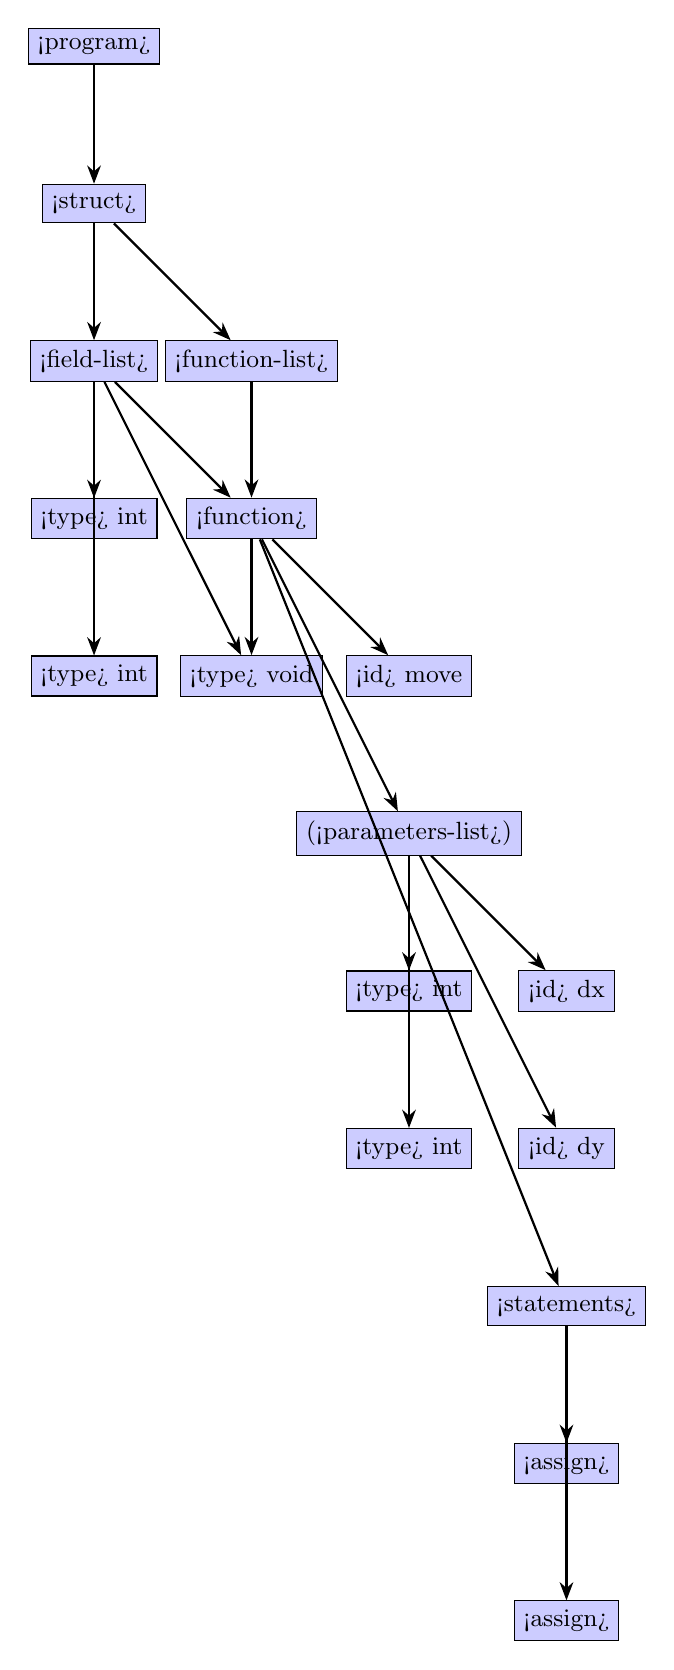
\begin{tikzpicture}[
	node distance=2cm,
	every node/.style={draw, fill=blue!20, text centered, font=\small},
	function/.style={draw, fill=orange!20, text centered, font=\small},
	edge/.style={draw, thick, -Stealth}
	]
	
	% Define nodes
	\node (program) {<program>};
	\node (struct) [below of=program] {<struct>};
	\node (fieldList) [below of=struct] {<field-list>};
	\node (functionList) [right of=fieldList] {<function-list>};
	\node (type1) [below of=fieldList] {<type> int};
	\node (id1) [right of=type1] {<id> x};
	\node (type2) [below of=type1] {<type> int};
	\node (id2) [right of=type2] {<id> y};
	\node (function1) [below of=functionList] {<function>};
	\node (type3) [below of=function1] {<type> void};
	\node (id3) [right of=type3] {<id> move};
	\node (parameters) [below of=id3] {(<parameters-list>)};
	\node (param1) [below of=parameters] {<type> int};
	\node (param2) [right of=param1] {<id> dx};
	\node (param3) [below of=param1] {<type> int};
	\node (param4) [right of=param3] {<id> dy};
	\node (statements) [below of=param4] {<statements>};
	\node (assign1) [below of=statements] {<assign>};
	\node (assign2) [below of=assign1] {<assign>};
	
	% Draw edges
	\path [edge] (program) -- (struct);
	\path [edge] (struct) -- (fieldList);
	\path [edge] (fieldList) -- (type1);
	\path [edge] (fieldList) -- (id1);
	\path [edge] (fieldList) -- (type2);
	\path [edge] (fieldList) -- (id2);
	\path [edge] (struct) -- (functionList);
	\path [edge] (functionList) -- (function1);
	\path [edge] (function1) -- (type3);
	\path [edge] (function1) -- (id3);
	\path [edge] (function1) -- (parameters);
	\path [edge] (parameters) -- (param1);
	\path [edge] (parameters) -- (param2);
	\path [edge] (parameters) -- (param3);
	\path [edge] (parameters) -- (param4);
	\path [edge] (function1) -- (statements);
	\path [edge] (statements) -- (assign1);
	\path [edge] (statements) -- (assign2);
	
\end{tikzpicture}
\section{تقدم عملگر‌ها}


ترتیب و نحوه ارزیابی عملگر‌ها به دو مفهوم تقدم (\lr{Precedence}) و وابستگی (\lr{Associativity}) عملگر‌ها 
وابسته است. هر دو این مفاهیم مرتبط با زمان کامپایل کد هستند.
تقدم عملگرها مشخص می‌کند که در یک عبارت که شامل چندین عملگر است، کدام عملگر ابتدا اجرا شود و وابستگی عملگرها مشخص می‌کند که اگر چندین عملگر با تقدم یکسان در یک عبارت وجود داشته باشند، کدام یک ابتدا ارزیابی شوند.

\begin{figure}[h!]
	\centering
	%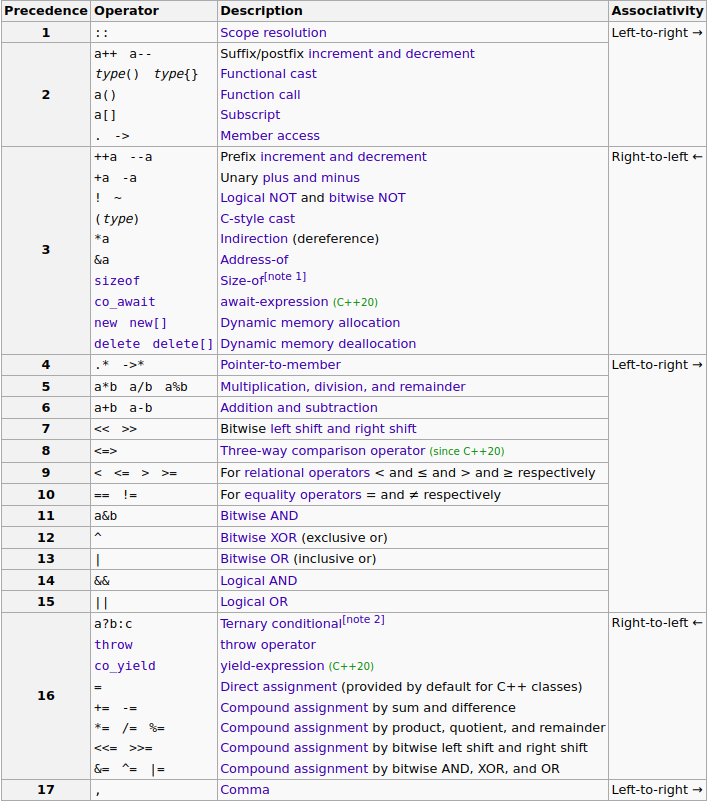
\includegraphics[width=\textwidth]{img/1-operations.png}
	\caption{تمام عملگرهای زبان \lr{C++} به همراه تقدم و وابستگی}
	\label{fig:example}
\end{figure}

تقدم عملگر‌ها با بارگذاری بیش از حد عملگر‌ها (\lr{operator overloading}) تغییری نمی‌کند و ثابت خواهد ماند.
برای نمونه در مثال زیر نحوه ارزیابی مشخص شده است.

\begin{LTR} % Left-to-right environment for code
	\begin{lstlisting}
		cout << a ? b : c;
	\end{lstlisting}
\end{LTR}

\begin{LTR} % Left-to-right environment for code
	\begin{lstlisting}
		(cout << a) ? b : c;
	\end{lstlisting}
\end{LTR}
\section{گرامر بدون ابهام رعایت تقدم عملگر‌ها}

\begin{table}[h!]
	\centering
	\begin{tabular}{|c|c|}
		\hline
		\textbf{عملگرها} & \textbf{تقدم} \\
		\hline
		\texttt{\&\&}, \texttt{||} & 5 \\
		\hline
		\texttt{\&}, \texttt{|} & 4 \\
		\hline
		\texttt{+}, \texttt{-} & 3 \\
		\hline
		\texttt{*}, \texttt{/} & 2 \\
		\hline
		\texttt{a++}, \texttt{a--} & 1 \\
		\hline
	\end{tabular}
	\caption{تقدم عملگرها در زبان C++}
	\label{tab:operator_precedence}
\end{table}

\begin{align*}
	\langle \text{id} \rangle &\to A \mid B \mid C \mid D \mid \dots \\
	\langle \text{assign} \rangle &\to \langle \text{id} \rangle = \langle \text{logical-or} \rangle \\
	\langle \text{logical-or} \rangle &\to \langle \text{logical-or} \rangle \, || \, \langle \text{logical-and} \rangle \mid \langle \text{logical-or} \rangle \\
	\langle \text{logical-and} \rangle &\to \langle \text{logical-and} \rangle \, && \, \langle \text{bitwise-or} \rangle \mid \langle \text{bitwise-or} \rangle \\
	\langle \text{bitwise-or} \rangle &\to \langle \text{bitwise-or} \rangle \, | \, \langle \text{bitwise-and} \rangle \mid \langle \text{bitwise-and} \rangle \\
	\langle \text{bitwise-and} \rangle &\to \langle \text{bitwise-and} \rangle \, \& \, \langle \text{additive} \rangle \mid \langle \text{additive} \rangle \\
	\langle \text{additive} \rangle &\to \langle \text{additive} \rangle \, (+, -) \, \langle \text{multiplicative} \rangle \mid \langle \text{multiplicative} \rangle \\
	\langle \text{multiplicative} \rangle &\to \langle \text{multiplicative} \rangle \, (*, /) \, \langle \text{factor} \rangle \mid \langle \text{factor} \rangle \\
	\langle \text{factor} \rangle &\to (\langle \text{logical-or} \rangle) \mid \langle \text{id} \rangle \mid \langle \text{id} \rangle++ \mid \langle \text{id} \rangle--
\end{align*}
\section{معناشناسی عملیاتی بعضی از ساختارها}

\subsection{تخصیص مقدار به متغیر}
\begin{LTR} % Left-to-right environment for code
	\begin{lstlisting}[breaklines=true]
		x = 5;
		
		MOV R1, #5      ; Load the constant 5 into register R1
		MOV [x], R1     ; Store the value of R1 into memory at
		the address of x
	\end{lstlisting}
\end{LTR}

\subsection{جمع دو مقدار}
\begin{LTR} % Left-to-right environment for code
	\begin{lstlisting}[breaklines=true]
		z = x + y;
		
		MOV R1, [x]     ; Load the value of x into register R1
		MOV R2, [y]     ; Load the value of y into register R2
		ADD R3, R1, R2  ; Add the values in R1 and R2, store 
		the result in R3
		MOV [z], R3     ; Store the result in memory location z
	\end{lstlisting}
\end{LTR}

\subsection{شرط ساده \lr{(if-else)}}
\begin{LTR} % Left-to-right environment for code
	\begin{lstlisting}[breaklines=true]
		if (x > 0) {
			y = 1;
		} else {
			y = -1;
		}
		
		MOV R1, [x]      ; Load x into R1
		CMP R1, #0       ; Compare R1 with 0
		JLE ELSE_LABEL   ; Jump to ELSE_LABEL if R1 <= 0
		MOV [y], #1      ; If x > 0, assign 1 to y
		JMP END_LABEL    ; Skip the else branch
		ELSE_LABEL:
		MOV [y], #-1     ; If x <= 0, assign -1 to y
		END_LABEL:
	\end{lstlisting}
\end{LTR}


\subsection{حلقه \lr{(while)}}
\begin{LTR} % Left-to-right environment for code
	\begin{lstlisting}[breaklines=true]
		while (x > 0) {
			x = x - 1;
		}
		
		
		LOOP_LABEL:
		MOV R1, [x]      ; Load x into R1
		CMP R1, #0       ; Compare R1 with 0
		JLE END_LABEL    ; Exit the loop if R1 <= 0
		SUB R1, R1, #1   ; Decrement R1 by 1
		MOV [x], R1      ; Update x in memory
		JMP LOOP_LABEL   ; Repeat the loop
		END_LABEL:
	\end{lstlisting}
\end{LTR}


\subsection{حلقه \lr{(for)}}
\begin{LTR} % Left-to-right environment for code
	\begin{lstlisting}[breaklines=true]
		for (int i = 0; i < 5; i++) {
			sum = sum + i;
		}
		
		
		; Initialize the loop counter i = 0
		MOV R1, #0        ; Load 0 into R1 (i = 0)
		MOV [i], R1       ; Store the value of i in memory
		
		; Initialize sum = 0
		MOV R2, #0        ; Load 0 into R2 (sum = 0)
		MOV [sum], R2     ; Store the value of sum in memory
		
		FOR_LOOP_START:
		; Compare i with the upper limit (5)
		MOV R1, [i]       ; Load the current value of i into R1
		CMP R1, #5        ; Compare i with 5
		JGE FOR_LOOP_END  ; If i >= 5, jump to end of the loop
		
		; Add i to sum
		MOV R2, [sum]     ; Load the current value of sum into R2
		ADD R2, R2, R1    ; Compute sum + i
		MOV [sum], R2     ; Store the updated sum back into memory
		
		; Increment i by 1
		MOV R1, [i]       ; Load the current value of i into R1
		ADD R1, R1, #1    ; Increment i by 1
		MOV [i], R1       ; Store the updated value of i in memory
		
		; Jump back to the start of the loop
		JMP FOR_LOOP_START
		
		FOR_LOOP_END:
		; End of the loop
	\end{lstlisting}
\end{LTR}


\subsection{تعریف و فراخوانی تابع}
\begin{LTR} % Left-to-right environment for code
	\begin{lstlisting}[breaklines=true]
		int add(int a, int b) {
			return a + b;
		}
		
		int result = add(3, 4);
		
		
		; Define the function
		ADD_FUNC:
		PUSH R1          ; Save registers
		PUSH R2
		ADD R3, R1, R2   ; Compute a + b, store result in R3
		POP R2           ; Restore registers
		POP R1
		RET              ; Return from the function
		
		; Call the function
		MOV R1, #3       ; Pass 3 as the first argument (in R1)
		MOV R2, #4       ; Pass 4 as the second argument (in R2)
		CALL ADD_FUNC    ; Call the add function
		MOV [result], R3 ; Store the result in memory
	\end{lstlisting}
\end{LTR}


\subsection{استراکت}
\begin{LTR} % Left-to-right environment for code
	\begin{lstlisting}[breaklines=true]
		struct Point {
			int x;
			int y;
		};
		
		int main() {
			Point p;
			p.x = 5;
			p.y = 10;
			return 0;
		}
		
		
		main:
		pushq   %rbp                # Save base pointer
		movq    %rsp, %rbp          # Set stack frame
		subq    $16, %rsp           # Allocate 16 bytes on 
		the stack for 'p'
		
		movl    $5, -8(%rbp)        # Set p.x = 5
		movl    $10, -4(%rbp)       # Set p.y = 10
		
		movl    $0, %eax            # Return 0
		leave                       # Restore base pointer
		ret                         # Return
	\end{lstlisting}
\end{LTR}
\chapter{متغیرها و نوع‌های داده‌ای}
\section{انقیاد}

\subsection{انقیاد نوع}
انقیاد نوع به معنی این است که نوع یک متغیر در چه زمانی و چگونه تعیین می‌‌شود. زبان \lr{C++} یک زبان انقیاد نوع ایستا است اما در سناریو‌هایی مانند پلی مورفیسم از انقیاد نوع پویا نیز پشتیبانی می‌کند.

\subsubsection{انقیاد نوع ایستا در \lr{C++}}
\begin{itemize}
	\item نوع متغیر در زمان کامپایل مشخص می‌شود.
	\item خطاهای مرتبط با نوع در زمان کامپایل بررسی می‌شود.
	\item به دلیل تعیین خطاها و تشخیص نوع‌ها در زمان کامپایل زمان اجرا پایین است.
\end{itemize}

زبان C++ روش‌های مختلفی برای استفاده از این نوع تعریف کرده است:
\begin{itemize}
	\item تعریف متغیر‌ها در برنامه
	\begin{LTR} % Left-to-right environment for code
		\begin{lstlisting}[breaklines=true]
			int num = 10;        // `num` is bound to type 
			`// int` at compile-time.
			double pi = 3.14;    // `pi` is bound to type 
			`// double` at compile-time.
			char ch = 'A';       // `ch` is bound to type `
			// char` at compile-time.
		\end{lstlisting}
	\end{LTR}
	
	
	\item تعریف توابع عادی در برنامه
	\begin{LTR} % Left-to-right environment for code
		\begin{lstlisting}[breaklines=true]
			void print(int value) {
				std::cout << "Integer: " << value << std::endl;
			}
			
			void print(double value) {
				std::cout << "Double: " << value << std::endl;
			}
			
			void print(const char* value) {
				std::cout << "String: " << value << std::endl;
			}
			
			int main() {
				print(10);               // Resolves to print(int)
				print(3.14);             // Resolves to print(double)
				print("Hello World");    // Resolves to print(const char*)
				return 0;
			}
		\end{lstlisting}
	\end{LTR}
	
	
	\item بارگذاری عملگرها
	\begin{LTR} % Left-to-right environment for code
		\begin{lstlisting}[breaklines=true]
			class Complex {
				public:
				double real, imag;
				
				Complex(double r, double i) : real(r), imag(i) {}
				
				Complex operator+(const Complex& c) {
					return Complex(real + c.real, imag + c.imag);
				}
			};
			
			int main() {
				Complex c1(1.0, 2.0), c2(3.0, 4.0);
				Complex c3 = c1 + c2;    // Operator `+` resolved at compile-time
				
				std::cout << "Real: " << c3.real << ", Imaginary: " << c3.imag << std::endl;
				return 0;
			}
			
		\end{lstlisting}
	\end{LTR}
	
	
	\item قالب‌های توابع (\lr{Function Templates})
	\begin{LTR} % Left-to-right environment for code
		\begin{lstlisting}[breaklines=true]
			template <typename T>
			T add(T a, T b) {
				return a + b;
			}
			
			int main() {
				std::cout << add(3, 4) << std::endl;         // Instantiates add<int>
				std::cout << add(3.14, 1.86) << std::endl;  // Instantiates add<double>
				return 0;
			}
		\end{lstlisting}
	\end{LTR}
	
	
	\item توابع خطی (\lr{inline})
	\begin{LTR} % Left-to-right environment for code
		\begin{lstlisting}[breaklines=true]
			inline int square(int x) {
				return x * x;
			}
			
			int main() {
				std::cout << square(5) << std::endl;   // `square(5)` is replaced with `5 * 5` at compile-time
				return 0;
			}
		\end{lstlisting}
	\end{LTR}
	
	
	\item عبارات ثابت
	\begin{LTR} % Left-to-right environment for code
		\begin{lstlisting}[breaklines=true]
			constexpr int square(int x) {
				return x * x;
			}
			
			int main() {
				constexpr int result = square(5);  // Computed at compile-time
				std::cout << result << std::endl;
				return 0;
			}
		\end{lstlisting}
	\end{LTR}
	
	
	
	\item توابع کلاس‌ها
	\begin{LTR} % Left-to-right environment for code
		\begin{lstlisting}[breaklines=true]
			class Base {
				public:
				void display() {
					std::cout << "Base class display" << std::endl;
				}
			};
			
			class Derived : public Base {
				public:
				void display() {
					std::cout << "Derived class display" << std::endl;
				}
			};
			
			int main() {
				Base obj;
				obj.display();   // Resolves to Base::display() at compile-time
				return 0;
			}
		\end{lstlisting}
	\end{LTR}
	
	\item عبارت‌های لامبدا
	\begin{LTR} % Left-to-right environment for code
		\begin{lstlisting}[breaklines=true]
			int main() {
				auto add = [](int a, int b) { return a + b; };  // Resolved at compile-time
				std::cout << add(3, 4) << std::endl;
				return 0;
			}
		\end{lstlisting}
	\end{LTR}
	
\end{itemize}


\subsubsection{انقیاد نوع پویا در \lr{C++}}
\begin{itemize}
	\item نوع متغیر در زمان اجرا مشخص می‌شود.
	\item خطاهای مرتبط با نوع در زمان اجرا بررسی می‌شود.
	\item به دلیل تعیین خطاها و تشخیص نوع‌ها در زمان اجرا زمان اجرا بالا است.
\end{itemize}

زبان \lr{C++} به دلیل زمان اجرای پایین این نوع انقیاد روش‌ محدودی را برای استفاده از این نوع تعریف کرده است و آن هم استفاده از توابع مجازی است.

\begin{LTR} % Left-to-right environment for code
	\begin{lstlisting}[breaklines=true]
		class Base {
			public:
			virtual void display() {  // Virtual function enables dynamic binding
				std::cout << "Base class display" << std::endl;
			}
		};
		
		class Derived : public Base {
			public:
			void display() override {  // Overrides the base class method
				std::cout << "Derived class display" << std::endl;
			}
		};
		
		int main() {
			Base* basePtr;
			Derived derivedObj;
			basePtr = &derivedObj;
			
			basePtr->display();  // Resolved at runtime to Derived::display
			return 0;
		}
	\end{lstlisting}
\end{LTR}


\begin{LTR} % Left-to-right environment for code
	\begin{lstlisting}[breaklines=true]
		class Animal {
			public:
			virtual void speak() = 0;  // Pure virtual function
		};
		
		class Dog : public Animal {
			public:
			void speak() override {
				std::cout << "Woof!" << std::endl;
			}
		};
		
		class Cat : public Animal {
			public:
			void speak() override {
				std::cout << "Meow!" << std::endl;
			}
		};
		
		int main() {
			Animal* animal;
			
			Dog dog;
			Cat cat;
			
			animal = &dog;
			animal->speak();  // Resolved at runtime to Dog::speak
			
			animal = &cat;
			animal->speak();  // Resolved at runtime to Cat::speak
			
			return 0;
		}
	\end{lstlisting}
\end{LTR}
\section{مقایسه انقیاد ایستا و پویا}

\begin{table}[h!]
	\centering
	\begin{tabular}{|p{3cm}|p{5cm}|p{5cm}|}
		\hline
		\textbf{ویژگی} & \textbf{انقیاد ایستا} & \textbf{انقیاد پویا} \\
		\hline
		زمان حل اتصال & زمان کامپایل & زمان اجرا \\
		\hline
		عملکرد & بالا (بدون سربار در زمان اجرا) & کمی کندتر (سربار جدول مجازی و\lr{ RTTI}) \\
		\hline
		تشخیص خطا & در زمان کامپایل (ایمن‌تر) & در زمان اجرا (کمتر ایمن) \\
		\hline
		انعطاف‌پذیری & محدود (نوع‌ها در زمان کامپایل ثابت هستند) & بالا (پشتیبانی از چندریختی در زمان اجرا) \\
		\hline
		قابلیت گسترش & نیاز به بازکامپایل برای تغییرات & راحت برای گسترش (مثلاً اضافه کردن کلاس‌های جدید) \\
		\hline
		سهولت در دیباگ & آسان‌تر (رفتار قابل پیش‌بینی است) & دشوارتر (رفتار وابسته به زمان اجرا است) \\
		\hline
		استفاده از حافظه & کم (نیاز به فراداده اضافی نیست) & بیشتر (نیاز به جدول مجازی و \lr{RTTI}) \\
		\hline
		موارد استفاده & کدهای کارآمد و قابل پیش‌بینی (مثل الگوریتم‌ها) & طراحی انعطاف‌پذیر و قابل گسترش (مثل فریم‌ورک‌ها) \\
		\hline
	\end{tabular}
	\caption{مقایسه انقیاد ایستا و پویا}
	\label{tab:static_dynamic_binding}
\end{table}

\subsection{انقیاد مقدار یا حافظه}
انقیاد مقدار به معنی این است که نوع یک متغیر در چه زمانی و چگونه به حافظه مقید می‌‌شود. 
زبان\lr{ C++} از انواع زیر پشتیبانی می‌کند:


\subsubsection{انقیاد در زمان کامپایل}
\begin{itemize}
	\item آدرس حافظه در زمان کامپایل تعیین می‌شود.
	\item این نوع انقیاد در زبان \lr{C++ }مرسوم‌‌تر است و برای متغیر‌های محلی و سراسری و ایستا استفاده می‌شود.
	
	\begin{LTR} % Left-to-right environment for code
		\begin{lstlisting}[breaklines=true]
			int x = 10;
			static int y = 0;
		\end{lstlisting}
	\end{LTR}
\end{itemize}


\subsubsection{انقیاد در زمان اجرا}
\begin{itemize}
	\item آدرس حافظه در زمان اجرا مشخص می‌شود.
	\item برنامه‌نویس مسئول آزاد کردن حافظه است.
	\item این نوع انقیاد معمولاً در تخصیص پویا (\lr{Dynamic Allocation}) با استفاده از دستوراتی مانند \lr{new} انجام می‌شود.
	
	
	\begin{LTR} % Left-to-right environment for code
		\begin{lstlisting}
			int* ptr = new int(10);
		\end{lstlisting}
	\end{LTR}
\end{itemize}


\subsubsection{انقیاد موقت}
\begin{itemize}
	\item حافظه به صورت موقت رزرو می‌شود.
	\item این نوع انقیاد زمانی رخ می‌دهد که یک مقدار موقت (\lr{temporary}) به یک مرجع متصل شود. این اتصال تا زمانی که مرجع در محدوده است، معتبر باقی می‌ماند.
	
	
	\begin{LTR} % Left-to-right environment for code
		\begin{lstlisting}
			const int& ref = 42;
		\end{lstlisting}
	\end{LTR}
\end{itemize}


\subsubsection{انقیاد پویا با اشاره‌گرهای هوشمند}
\begin{itemize}
	\item آزادسازی حافظه به صورت خودکار توسط اشاره‌گر هوشمند انجام می‌شود.
	\item در \lr{C++} مدرن (11 به بعد)، از اشاره‌گرهای هوشمند برای مدیریت انقیاد حافظه به صورت خودکار استفاده می‌شود.
\end{itemize}

\begin{LTR} % Left-to-right environment for code
	\begin{lstlisting}[breaklines=true]
		std::unique_ptr<int> ptr = std::make_unique<int>(10);
	\end{lstlisting}
\end{LTR}


\section{تعریف متغیر}
در زبان \lr{C++ }تعریف متغیر صریح مرسوم است اما ابزاری برای تعریف متغیر ضمنی نیز وجود دارد.

\subsection{تعریف متغیر صریح}
نوع متغیر به‌طور واضح و صریح در هنگام تعریف مشخص می‌شود.

\begin{LTR} % Left-to-right environment for code
	\begin{lstlisting}[breaklines=true]
		int age = 25;          // 'age' is explicitly defined as an integer.
		double pi = 3.14;      // 'pi' is explicitly defined as a double.
		string name = "John";  // 'name' is explicitly defined as a string.
	\end{lstlisting}
\end{LTR}

\subsection{تعریف متغیر ضمنی}
نوع متغیر برابر با \lr{auto} قرار می‌گیرد و نوع به‌طور خودکار توسط کامپایلر با توجه به مقدار زمینه تعیین می‌شود.

\begin{LTR} % Left-to-right environment for code
	\begin{lstlisting}[breaklines=true]
		auto age = 25;         // The type of 'age' is inferred as int.
		auto pi = 3.14;        // The type of 'pi' is inferred as double.
		auto name = "John";    // The type of 'name' is inferred as const char*.
	\end{lstlisting}
\end{LTR}

\begin{table}[h!]
	\centering
	\begin{tabular}{|p{3cm}|p{5cm}|p{5cm}|}
		\hline
		\textbf{ویژگی} & \textbf{تعریف صریح} & \textbf{تعریف ضمنی} \\
		\hline
		وضوح & 
		نوع متغیر به‌طور واضح و مستقیم مشخص می‌شود. & 
		نوع متغیر توسط کامپایلر استنباط می‌شود و ممکن است بلافاصله واضح نباشد. \\
		\hline
		انعطاف‌پذیری & 
		نیاز به دانستن نوع متغیر قبل از تعریف دارد. & 
		می‌تواند براساس مقدار داده شده، نوع را تطبیق دهد. \\
		\hline
		نحو (\lr{Syntax}) & 
		روش سنتی و نسبتاً طولانی. & 
		کوتاه‌تر و مدرن‌تر با استفاده از \texttt{\lr{auto}}. \\
		\hline
		مورد استفاده & 
		مناسب برای مواردی که وضوح و کنترل اهمیت دارند. & 
		مناسب برای کاهش کد تکراری، مخصوصاً در انواع پیچیده. \\
		\hline
	\end{tabular}
	\caption{مقایسه تعریف صریح و تعریف ضمنی متغیرها در زبان C++}
	\label{tab:explicit_implicit}
\end{table}


\section{متغیرهای ایستا}

\subsection{متغیرهای ایستا در توابع}
\begin{itemize}
	\item مقدار آن بین فراخوانی‌های مختلف تابع حفظ می‌شود.
	\item فقط یک بار مقداردهی اولیه می‌شود.
	\item مقدار آن پس از خروج از تابع باقی می‌ماند.
	\item دامنه (\lr{Scope}) متغیر همچنان محدود به تابع است، اما طول عمر (\lr{Lifetime}) آن برابر با طول عمر برنامه خواهد بود.
	\item در قسمت دیتا سگمنت ذخیره می‌شود.
\end{itemize}


\begin{LTR} % Left-to-right environment for code
	\begin{lstlisting}[breaklines=true]
		void countCalls() {
			static int count = 0; // متغیر استاتیک
			count++;
			cout << "This function has been called " << count << " times." << endl;
		}
		
		int main() {
			countCalls();
			countCalls();
			countCalls();
			return 0;
		}
	\end{lstlisting}
\end{LTR}

خروجی:

\begin{LTR} % Left-to-right environment for code
	\begin{lstlisting}[breaklines=true]
		This function has been called 1 times.
		This function has been called 2 times.
		This function has been called 3 times.
	\end{lstlisting}
\end{LTR}


\subsection{متغیرهای ایستا در کلاس‌ها}
\begin{itemize}
	\item در داخل یک کلاس، متغیرهای استاتیک به همه اشیاء (\lr{Objects}) آن کلاس مشترک هستند. این متغیرها بخشی از فضای ذخیره‌سازی کلاس هستند، نه اشیاء جداگانه.
	\item مستقل از اشیاء کلاس هستند.
	\item فقط یک نسخه از آنها در حافظه وجود دارد که توسط تمام اشیاء به اشتراک گذاشته می‌شود.
	\item برای دسترسی به آنها می‌توان از نام کلاس استفاده کرد.
	\item در قسمت دیتا سگمنت ذخیره می‌شود.
\end{itemize}


\begin{LTR} % Left-to-right environment for code
	\begin{lstlisting}[breaklines=true]
		class Counter {
			private:
			static int count; // متغیر استاتیک
			public:
			Counter() {
				count++;
			}
			static void showCount() { // متد استاتیک
				cout << "Count: " << count << endl;
			}
		};
		
		int Counter::count = 0; // مقداردهی اولیه متغیر استاتیک
		
		int main() {
			Counter c1, c2, c3;
			Counter::showCount(); // دسترسی به متغیر استاتیک از طریق کلاس
			return 0;
		}
	\end{lstlisting}
\end{LTR}

خروجی:

\begin{LTR} % Left-to-right environment for code
	\begin{lstlisting}[breaklines=true]
		Count: 3
	\end{lstlisting}
\end{LTR}

\subsubsection{مزایا}
\begin{itemize}
	\item حفظ مقدار متغیر در توابع بدون نیاز به استفاده از متغیرهای سراسری.
	\item صرفه‌جویی در حافظه برای متغیرهای مشترک در بین اشیاء کلاس.
	\item امکان پیاده‌سازی شمارنده‌ها، حافظه پنهان (\lr{Cache}) و بسیاری از موارد دیگر.
\end{itemize}


\section{پویا در پشته}

\subsection{متغیر‌های محلی}
هنگام اجرای تابع حافظه تخصیص داده می‌شود و در پایان تابع آزاد می‌‌شوند.



\begin{LTR} % Left-to-right environment for code
	\begin{lstlisting}[breaklines=true]
		void myFunction() {
			int a = 10;  // Stored on the stack
		}
	\end{lstlisting}
\end{LTR}


\subsection{پارامتر‌های توابع}


\begin{LTR} % Left-to-right environment for code
	\begin{lstlisting}[breaklines=true]
		void printNumber(int num) {
			// num is stored on the stack
		}
	\end{lstlisting}
\end{LTR}

\subsubsection{آرایه‌‌های محلی غیر پویا}
\begin{LTR} % Left-to-right environment for code
	\begin{lstlisting}[breaklines=true]
		void myFunction() {
			int arr[5] = {1, 2, 3, 4, 5}; // روی پشته ذخیره می‌شود
		}
	\end{lstlisting}
\end{LTR}


\section{متغیرهای پویا در هیپ به طور صریح}

زبان C++ تعریف این متغیرها را ممکن ساخته است و برای این کار از دو عملگر \lr{new} (برای تخصیص حافظه) و عملگر \lr{delete} (برای آزاد کردن فضای تخصیص داده‌ شده) استفاده می‌کند.

\begin{itemize}
	\item حافظه‌ای که با new تخصیص داده شده باید حتماً با delete آزاد شود.
	\item آزاد نکردن حافظه منجر به نشت حافظه (\lr{memory leak}) می‌شود.
	\item استفاده از \lr{delete} برای حافظه‌ای که تخصیص نیافته یا قبلاً آزاد شده است، باعث رفتار غیرقابل پیش‌بینی خواهد شد.
\end{itemize}


\begin{LTR} % Left-to-right environment for code
	\begin{lstlisting}[breaklines=true]
		int* ptr = new int;
		int* arr = new int[5];
		Data* data = new Data(); // instance of class Data
	\end{lstlisting}
\end{LTR}


\section{متغیرهای پویا در هیپ به طور ضمنی}

زبان \lr{C++} امکان استفاده از این نوع متغیرها را نیز فراهم کرده است و از طریق اشاره‌گر‌های هوشمند و یا کتاب‌خانه‌های استاندارد و … از این روش استفاده می‌کند. همچنین در این روش متغیر‌ها در بخش هیپ ذخیره می‌شوند اما ابزار‌های آماده حافظه را به‌‌صورت خودکار مدیریت می‌‌‌کنند.


\subsection{اشاره‌گرهای هوشمند}


\begin{LTR} % Left-to-right environment for code
	\begin{lstlisting}[breaklines=true]
		#include <memory> // For smart pointers
		
		int main() {
			// Define a shared_ptr to manage a dynamic integer
			std::shared_ptr<int> ptr = std::make_shared<int>(42);
			
			std::cout << "Value: " << *ptr << std::endl;
			
			// Memory is automatically freed when it goes out of scope
			
			return 0;
		}
	\end{lstlisting}
\end{LTR}

\subsubsection{کانتینرهای STL}
\begin{LTR} % Left-to-right environment for code
	\begin{lstlisting}[breaklines=true]
		#include <vector>
		
		int main() {
			// Define a vector of integers
			std::vector<int> numbers = {1, 2, 3, 4, 5};
			
			// Add an element to the vector
			numbers.push_back(6);
			
			// Print the values of the vector
			for (int num : numbers) {
				std::cout << num << " ";
			}
			std::cout << std::endl;
			
			// No need to free memory; it is managed automatically
			
			return 0;
		}
	\end{lstlisting}
\end{LTR}


\begin{table}[h!]
	\centering
	\begin{tabular}{|p{4cm}|p{6cm}|p{6cm}|}
		\hline
		\textbf{نوع متغیر} & \textbf{مزایا} & \textbf{معایب} \\
		\hline
		ایستا &
		\begin{itemize}
			\item تخصیص حافظه ثابت در طول عمر برنامه.
			\item حفظ مقدار بین اجرای توابع.
			\item بدون سربار حافظه در زمان اجرا.
		\end{itemize} &
		\begin{itemize}
			\item حافظه در طول عمر برنامه اشغال می‌شود، حتی اگر به ندرت استفاده شود.
			\item ممکن است باعث افزایش غیرضروری حافظه شود.
		\end{itemize} \\
		\hline
		پویا در پشته &
		\begin{itemize}
			\item مناسب برای مقادیر ثابت یا مقادیری که به ندرت تغییر می‌کنند.
			\item تخصیص و آزادسازی خودکار (بر اساس محدوده متغیر).
			\item تخصیص و آزادسازی سریع (روی پشته).
			\item امنیت بالا.
		\end{itemize} &
		\begin{itemize}
			\item نمی‌توانند خارج از محدوده تابع باقی بمانند.
		\end{itemize} \\
		\hline
		پویا در هیپ به طور صریح &
		\begin{itemize}
			\item انعطاف‌پذیری: اندازه حافظه در زمان اجرا تعیین می‌شود.
			\item مناسب برای داده‌های بزرگ و پویا.
			\item کنترل دستی بر طول عمر حافظه فراهم می‌کند.
		\end{itemize} &
		\begin{itemize}
			\item نیازمند تخصیص دستی (\texttt{new}) و آزادسازی دستی (\texttt{delete}).
			\item احتمال نشت حافظه در صورت آزاد نکردن صحیح.
			\item خطر رفتار غیرقابل پیش‌بینی در صورت آزادسازی دوباره یا دسترسی پس از آزادسازی.
		\end{itemize} \\
		\hline
		پویا در هیپ به طور ضمنی &
		\begin{itemize}
			\item مدیریت خودکار حافظه (مانند کانتینرهای STL یا اشاره‌گرهای هوشمند).
			\item کاهش خطر نشت حافظه و رفتار غیرقابل پیش‌بینی.
			\item ساده کردن برنامه‌نویسی برای مفاهیم سطح بالا.
		\end{itemize} &
		\begin{itemize}
			\item کمی سربار عملکرد به دلیل مدیریت خودکار حافظه.
			\item کنترل کمتری بر تخصیص و آزادسازی حافظه.
			\item ممکن است در برنامه‌های حساس به عملکرد که هر تخصیص اهمیت دارد، بهینه نباشد.
		\end{itemize} \\
		\hline
	\end{tabular}
	\caption{مقایسه روش‌های تخصیص حافظه}
	\label{tab:memory_allocation}
\end{table}

\subsection{مقایسه سرعت انواع متغیرها}
\begin{table}[H]
	\centering
	\begin{tabular}{|p{4cm}|p{3cm}|p{7cm}|}
		\hline
		\textbf{نوع متغیر} & \textbf{سرعت} & \textbf{دلیل} \\
		\hline
		ایستا &
		بدون هزینه در زمان اجرا &
		این متغیرها در زمان کامپایل و در یک منطقه ثابت حافظه تخصیص داده می‌شوند. نیازی به جستجو یا نگهداری در زمان اجرا نیست. \\
		\hline
		پویا در پشته &
		سریع‌ترین &
		تخصیص در استک یک فرآیند ساده است که فقط اشاره‌گر حافظه را افزایش یا کاهش می‌دهد. نیازی به نگهداری پیچیده نیست. \\
		\hline
		پویا در هیپ به طور صریح &
		کندترین &
		هیپ یک فضای حافظه بزرگ و نامرتب است که نیاز به نگهداری پیچیده‌ای دارد. سیستم‌عامل یا زمان اجرا باید یک بلوک آزاد مناسب برای تخصیص پیدا کند. سربار شامل جستجوی حافظه، به‌روزرسانی ساختارهای داده داخلی و تضمین ایمنی رشته‌ها است. \\
		\hline
		پویا در هیپ به طور ضمنی &
		متوسط &
		حافظه هنوز روی هیپ تخصیص داده می‌شود، اما زمان اجرا از تکنیک‌هایی مانند اشاره‌گرهای ساده یا مجموعه‌های حافظه استفاده می‌کند. این فرآیند از تخصیص صریح کمی سریع‌تر است چون برنامه به طور مستقیم با توابع تخصیص سطح پایین درگیر نمی‌شود. فرآیند جمع‌آوری زباله (\lr{garbage collection}) سربار اضافی در آینده ایجاد می‌کند. \\
		\hline
	\end{tabular}
	\caption{مقایسه سرعت و دلایل تخصیص حافظه}
	\label{tab:memory_speed}
\end{table}
\pagebreak
\section{حوزه تعریف }
\subsection{حوزه تعریف ایستا \lr{(Static Scope)} در \lr{C++}}
در \lr{C++}، هر متغیر یا تابع در حوزه‌ای خاص تعریف می‌شود و دسترسی به آن‌ها از خارج از آن حوزه امکان‌پذیر نیست. این حوزه‌ها معمولاً در زمان کامپایل مشخص می‌شوند و شامل دو نوع اصلی هستند:

\subsubsection{حوزه تعریف درون توابع \lr{(Local Scope)}}
متغیرهایی که در داخل توابع یا بلوک‌ها تعریف می‌شوند، تنها در آن تابع یا بلوک قابل دسترسی هستند. این نوع متغیرها در زمان اجرای برنامه تنها در محدوده‌ای که تعریف شده‌اند معتبر هستند و پس از خروج از آن حوزه از بین می‌روند.

\textbf{مثال 1: متغیر محلی در یک تابع}
\LTR
\begin{lstlisting}[language=C++,breaklines=true]
	#include <iostream>
	
	void exampleFunction() {
		int x = 10; // access just here
		std::cout << "x = " << x << std::endl;
	}
	
	int main() {
		exampleFunction();
		// std::cout << x;  // error
		return 0;
	}
\end{lstlisting}
\RTL

در این مثال، متغیر \lr{x} تنها درون تابع \lr{exampleFunction} تعریف شده است و دسترسی به آن از خارج از تابع مجاز نیست.

\subsubsection{حوزه تعریف سراسری \lr{(Global Scope)}}
متغیرهایی که خارج از توابع و کلاس‌ها، در سطح کل برنامه تعریف می‌شوند، در تمام برنامه قابل دسترسی هستند. این متغیرها معمولاً از نوع \lr{global} هستند و در تمامی توابع یا کلاس‌ها می‌توانند استفاده شوند (به شرطی که در ابتدای برنامه تعریف شده باشند).

\textbf{مثال 2: متغیر سراسری}
\LTR
\begin{lstlisting}[language=C++, breaklines=true]
	#include <iostream>
	
	int globalVar = 5; // global
	
	void printGlobalVar() {
		std::cout << "globalVar = " << globalVar << std::endl; // access to global
	}
	
	int main() {
		printGlobalVar();
		return 0;
	}
\end{lstlisting}
\RTL

در این مثال، متغیر \lr{globalVar} در سطح سراسری برنامه تعریف شده است و می‌توان به آن از هر کجای برنامه مانند تابع \lr{printGlobalVar} دسترسی پیدا کرد.

\subsubsection{حوزه تعریف درون کلاس‌ها \lr{(Class Scope)}}
در \lr{C++}، متغیرها و توابعی که درون کلاس‌ها تعریف می‌شوند، تنها درون همان کلاس و از طریق شیءهای کلاس قابل دسترسی هستند.

\textbf{مثال 3: متغیر و تابع در کلاس}
\LTR
\begin{lstlisting}[language=C++, breaklines=true]
	#include <iostream>
	
	class MyClass {
		public:
		int value; /
		
		void printValue() { 
			std::cout << "value = " << value << std::endl;
		}
	};
	
	int main() {
		MyClass obj;
		obj.value = 10;
		obj.printValue(); 
		return 0;
	}
\end{lstlisting}
\RTL
در اینجا، متغیر \lr{value} و تابع \lr{printValue} درون کلاس \lr{MyClass} قرار دارند و تنها از طریق اشیاء این کلاس قابل دسترسی هستند.

\section{چالش‌ها و پیاده‌سازی حوزه تعریف پویا در \lr{C++}}
برای شبیه‌سازی حوزه تعریف پویا، نیاز است که متغیرهایی ایجاد شوند که بتوانند از توابع یا بلوک‌های مختلف و به‌صورت دینامیک قابل دسترسی باشند.

\textbf{مثال 1: پیاده‌سازی ساده با متغیر سراسری}
\LTR
\begin{lstlisting}[language=C++, breaklines=true]
#include <iostream>

int dynamicVar = 10;  // Global variable to simulate dynamic scoping

// First function that modifies the value of dynamicVar
void functionOne() {
	dynamicVar = 20;  // Modifying the value of dynamicVar in this function
	std::cout << "functionOne: dynamicVar = " << dynamicVar << std::endl;
}

// Second function that uses dynamicVar
void functionTwo() {
	std::cout << "functionTwo: dynamicVar = " << dynamicVar << std::endl;
}

int main() {
	std::cout << "main: dynamicVar = " << dynamicVar << std::endl;
	functionOne();  // Here, the value of dynamicVar is modified
	functionTwo();  // Here, the modified value of dynamicVar is displayed
	return 0;
}

\end{lstlisting}
\RTL

\textbf{خروجی برنامه:}
\LTR
\begin{verbatim}
	main: dynamicVar = 10
	functionOne: dynamicVar = 20
	functionTwo: dynamicVar = 20
\end{verbatim}
\RTL
در این مثال:
\begin{itemize}
	\item متغیر \lr{dynamicVar} که به‌طور سراسری تعریف شده است، ابتدا در تابع \lr{main} مقداردهی می‌شود.
	\item سپس در تابع \lr{functionOne}، مقدار آن به ۲۰ تغییر می‌کند.
	\item هنگامی که تابع \lr{functionTwo} فراخوانی می‌شود، مقدار تغییر یافته \lr{dynamicVar} نمایش داده می‌شود.
\end{itemize}
\subsection{استفاده از پشته (Stack) برای شبیه‌سازی حوزه پویا}
برای پیاده‌سازی واقعی‌تر حوزه پویا می‌توان از ساختارهای داده‌ای مانند پشته (\lr{stack}) استفاده کرد. این روش اجازه می‌دهد که مقادیر به صورت داینامیک ذخیره شوند و به ترتیب وارد و خارج شوند. به این ترتیب، متغیرها می‌توانند به طور پویا ذخیره و بازیابی شوند.

\textbf{مثال 2: استفاده از پشته برای ذخیره و بازیابی مقادیر}
\LTR
\begin{lstlisting}[language=C++,  breaklines=true]
	#include <iostream>
	#include <stack>
	
	// Stack to store variable values
	std::stack<int> dynamicStack;
	
	// Function to push a new value to the stack
	void functionOne() {
		dynamicStack.push(30);  // Add a new value to the stack
		std::cout << "functionOne: pushed 30" << std::endl;
	}
	// Function to retrieve the top value from the stack
	void functionTwo() {
		if (!dynamicStack.empty()) {
			int topValue = dynamicStack.top();  // Get the top value of the stack
			std::cout << "functionTwo: top of stack = " << topValue << std::endl;
			dynamicStack.pop();  // Remove the top value from the stack
		}
	}
	int main() {
		std::cout << "main: Initial stack is empty" << std::endl;
		functionOne();  // Add a new value to the stack
		functionTwo();  // Display the top value and remove it from the stack
		return 0;
	}
\end{lstlisting}
\RTL
\textbf{خروجی برنامه:}
\LTR
\begin{verbatim}
	main: Initial stack is empty
	functionOne: pushed 30
	functionTwo: top of stack = 30
\end{verbatim}
\RTL
در این مثال:
\begin{itemize}
	\item از پشته‌ای به نام \lr{dynamicStack} برای ذخیره مقادیر استفاده شده است.
	\item تابع \lr{functionOne} مقدار ۳۰ را به پشته اضافه می‌کند.
	\item تابع \lr{functionTwo} مقدار بالای پشته را خوانده و آن را از پشته برمی‌دارد.
\end{itemize}


\textbf{نتیجه‌گیری} \\
برای اضافه کردن حوزه تعریف پویا به زبان‌های ایستا مانند \lr{C++}، می‌توان از مکانیزم‌های مختلفی مانند متغیرهای سراسری یا ساختارهای داده‌ای دینامیک (مانند پشته) استفاده کرد. در این پیاده‌سازی، متغیرها می‌توانند در نقاط مختلف برنامه تغییر یافته و از هر کجا به آن‌ها دسترسی پیدا کرد، مشابه رفتار حوزه پویا که در زبان‌هایی مانند \lr{Lisp} مشاهده می‌شود.

\section{بلوک‌ها}
در زبان \lr{C++}، بلوک‌ها (\lr{Blocks}) معمولاً به عنوان مجموعه‌ای از دستورات محصور در آکولادها {} تعریف می‌شوند. این بلوک‌ها می‌توانند به‌عنوان بدنه‌ی توابع، حلقه‌ها، شروط و سایر ساختارهای کنترلی استفاده شوند. در این زبان، کلمات کلیدی خاصی برای تغییر حوزۀ تعریف متغیرها به‌طور مستقیم وجود ندارد، اما برای مدیریت دسترسی و تغییر حوزۀ متغیرها می‌توان از ویژگی‌های مختلف زبان مانند حوزه‌های محلی، حوزه‌های سراسری، و حوزه‌های ثابت بهره برد.

\subsection{تعریف بلوک‌ها در C++}
یک بلوک در \lr{C++} معمولاً به‌صورت مجموعه‌ای از دستورات نوشته می‌شود که بین آکولادها قرار دارند. بلوک‌ها می‌توانند در موقعیت‌های مختلفی قرار بگیرند، از جمله در داخل توابع، حلقه‌ها، و ساختارهای کنترلی مانند \lr{if} یا \lr{for}.

\textbf{مثال 1: تعریف بلوک در داخل یک تابع}
\LTR
\begin{lstlisting}[language=C++, breaklines=true]
	#include <iostream>
	
	void exampleFunction() {
		int x = 10;  // Variable x defined in this block
		{
			int y = 20;  // Variable y defined in this inner block
			std::cout << "Inside inner block: x = " << x << ", y = " << y << std::endl;
		}
		// std::cout << "y = " << y << std::endl; // Error: y is out of scope
	}
	
	int main() {
		exampleFunction();
		return 0;
	}
\end{lstlisting}
\RTL
در این مثال:
\begin{itemize}
	\item تابع \lr{exampleFunction} حاوی یک بلوک داخلی است که در داخل آن متغیر \lr{y} تعریف شده است. این متغیر تنها در داخل بلوک داخلی قابل دسترسی است.
	\item متغیر \lr{x} در داخل بلوک اصلی تابع تعریف شده و در داخل بلوک داخلی هم قابل دسترسی است.
\end{itemize}

\subsection{کلمات کلیدی ویژه برای اعمال تغییر در حوزه تعریف متغیرها}
در \lr{C++}، کلمات کلیدی خاصی برای تغییر مستقیم حوزه تعریف متغیرها وجود ندارد. اما چند ویژگی و کلمه کلیدی می‌توانند برای مدیریت دسترسی و کنترل حوزه متغیرها استفاده شوند:

\subsubsection{ \lr{auto}}
کلمه کلیدی \lr{auto} به کامپایلر این امکان را می‌دهد که نوع یک متغیر را به‌طور خودکار از مقدار آن استنتاج کند. این ویژگی به ساده‌سازی مدیریت حوزه متغیرها کمک می‌کند.

\textbf{مثال 2: استفاده از \lr{auto}}
\LTR
\begin{lstlisting}[language=C++, breaklines=true]
	#include <iostream>
	
	int main() {
		auto x = 5;  // Compiler infers x as int
		auto y = 10.5;  // Compiler infers y as double
		std::cout << "x = " << x << ", y = " << y << std::endl;
		return 0;
	}
\end{lstlisting}
\RTL

\subsubsection{ \lr{static}}
کلمه کلیدی \lr{static} برای حفظ مقدار متغیرها در تمام طول برنامه استفاده می‌شود. متغیرهای \lr{static} بین فراخوانی‌های متعدد یک تابع حفظ می‌شوند.

\textbf{مثال 3: استفاده از \lr{static}}
\LTR
\begin{lstlisting}[language=C++, breaklines=true]
	#include <iostream>
	
	void countCalls() {
		static int count = 0;  // Variable count persists across calls
		count++;
		std::cout << "Function called " << count << " times." << std::endl;
	}
	
	int main() {
		countCalls();
		countCalls();
		countCalls();
		return 0;
	}
\end{lstlisting}
\RTL
\subsubsection{\lr{extern}}
کلمه کلیدی \lr{extern} برای دسترسی به متغیرها یا توابع از فایل‌ها یا بخش‌های دیگر برنامه استفاده می‌شود. این کلمه امکان تعریف متغیرهای سراسری بین فایل‌ها را فراهم می‌کند.

\textbf{مثال 4: استفاده از \lr{extern}}
\LTR
\begin{lstlisting}[language=C++, breaklines=true]
	// File1.cpp
	#include <iostream>
	
	extern int globalVar;  // Declaration of global variable from another file
	
	void printGlobalVar() {
		std::cout << "Global Variable: " << globalVar << std::endl;
	}
	
	// File2.cpp
	int globalVar = 100;  // Definition of global variable
	
	int main() {
		printGlobalVar();
		return 0;
	}
\end{lstlisting}
\RTL
\subsubsection{\lr{const}}
کلمه کلیدی \lr{const} برای تعریف متغیرهایی استفاده می‌شود که مقدار آن‌ها ثابت و غیرقابل تغییر است. این کلمه کلیدی از تغییرات غیرمجاز جلوگیری می‌کند.

\textbf{مثال 5: استفاده از \lr{const}}
\LTR
\begin{lstlisting}[language=C++, breaklines=true]
	#include <iostream>
	
	void exampleFunction() {
		const int x = 5;  // Constant variable
		// x = 10;  // Error: Cannot modify a constant variable
		std::cout << "x = " << x << std::endl;
	}
	
	int main() {
		exampleFunction();
		return 0;
	}
\end{lstlisting}
\RTL

\textbf{نتیجه‌گیری} \\
\begin{itemize}
	\item در \lr{C++}، بلوک‌ها به‌صورت مجموعه‌ای از دستورات محصور در آکولادها \lr{\{\}} تعریف می‌شوند.
	\item برای مدیریت بهتر حوزه متغیرها می‌توان از کلمات کلیدی \lr{auto}، \lr{static}، \lr{extern} و \lr{const} استفاده کرد.
	\item این کلمات کلیدی به برنامه‌نویسان امکان مدیریت موثر حوزه، دسترسی و تغییرپذیری متغیرها را می‌دهند.
\end{itemize}
\section{نوع داده‌ها در زبان سی‌پلاس‌پلاس}

\subsection{انواع داده اولیه (\lr{Primary Data Types})}

\subsubsection{\texttt{int}}
\texttt{int} یک نوع داده برای ذخیره مقادیر عددی صحیح است. این نوع داده معمولاً برای ذخیره اعداد بدون قسمت اعشاری مانند شمارنده‌ها یا شاخص‌ها استفاده می‌شود. بسته به معماری سیستم، معمولاً ۴ بایت حافظه اشغال می‌کند.


\textbf{مثال:}
\LTR
\begin{lstlisting}
	// Store an integer named age
	int age = 25;
\end{lstlisting}
\RTL

\subsubsection{ \texttt{float}}
نوع داده \texttt{float} برای ذخیره اعداد اعشاری با دقت کم طراحی شده است. این نوع داده در محاسباتی که نیاز به دقت زیاد ندارند، مانند محاسبه تقریب‌های ریاضی یا متغیرهای عمومی در فیزیک و شیمی، به کار می‌رود.

\textbf{مثال:}
\LTR
\begin{lstlisting}
	// Store an approximate value of pi
	float pi = 3.14;
\end{lstlisting}
\RTL
\subsubsection{\texttt{double}}
نوع داده \texttt{double} برای ذخیره اعداد اعشاری با دقت بالا استفاده می‌شود. این نوع داده به دلیل ظرفیت بیشتر برای ذخیره اعداد و دقت بهتر در مقایسه با \texttt{float} معمولاً در محاسبات علمی و آماری به کار می‌رود.

\textbf{مثال:}
\LTR
\begin{lstlisting}
	// Store a precise decimal number
	double largeNumber = 123456.789;
\end{lstlisting}
\RTL
\subsubsection{ \texttt{char}}
نوع داده \texttt{char} برای ذخیره کاراکترها طراحی شده است. هر مقدار از این نوع داده معادل یک کد ASCII است که تنها یک بایت حافظه اشغال می‌کند. این نوع داده معمولاً در پردازش رشته‌ها یا نمایش کاراکترها استفاده می‌شود.

\textbf{مثال:}
\LTR
\begin{lstlisting}
	// Store a grade as a character
	char grade = 'A';
\end{lstlisting}
\RTL
\subsubsection{\texttt{bool}}
نوع داده \texttt{bool} برای ذخیره مقادیر منطقی \texttt{true} یا \texttt{false} استفاده می‌شود. این نوع داده در ساختارهای کنترلی مانند شرط‌ها و حلقه‌ها کاربرد گسترده‌ای دارد.

\textbf{مثال:}
\LTR
\begin{lstlisting}
	// Indicates whether the status is open or closed
	bool isOpen = true;
\end{lstlisting}
\RTL
\subsubsection{\texttt{void}}
نوع داده \texttt{void} برای توابعی استفاده می‌شود که هیچ مقداری را باز نمی‌گردانند. همچنین، این نوع داده برای تعریف اشاره‌گرهای کلی نیز به کار می‌رود که می‌توانند به هر نوع داده اشاره کنند.

\textbf{مثال:}
\LTR
\begin{lstlisting}
	// A function that only prints a message
	void greet() {
		cout << "Hello!";
	}
\end{lstlisting}
\RTL
\subsection{ انواع داده مشتق‌شده (\lr{Derived Data Types})}

\subsubsection{ آرایه (\lr{Array})}
آرایه مجموعه‌ای از عناصر با نوع داده یکسان است که به صورت پشت سر هم در حافظه ذخیره می‌شوند. آرایه‌ها برای ذخیره مجموعه‌ای از مقادیر مانند لیست اعداد یا کاراکترها استفاده می‌شوند.

\textbf{مثال:}
\LTR
\begin{lstlisting}
	// An array containing five integers
	int numbers[5] = {1, 2, 3, 4, 5};
\end{lstlisting}
\RTL
\subsubsection{ اشاره‌گر (\lr{Pointer})}
اشاره‌گر نوعی متغیر است که آدرس حافظه یک متغیر دیگر را ذخیره می‌کند. این نوع داده برای دسترسی مستقیم به حافظه و مدیریت پویا در برنامه‌ها به کار می‌رود.

\textbf{مثال:}
\LTR
\begin{lstlisting}
	// A pointer to the address of variable a
	int a = 10;
	int* p = &a;
\end{lstlisting}
\RTL
\subsubsection{ مرجع (\lr{Reference})}
مرجع یک نام مستعار برای متغیر دیگر است که به آن اجازه می‌دهد به صورت مستقیم به داده‌های متغیر اصلی دسترسی داشته باشد. این ویژگی اغلب در توابع برای جلوگیری از کپی کردن داده‌ها استفاده می‌شود.

\textbf{مثال:}
\LTR
\begin{lstlisting}
	// ref refers to x
	int x = 10;
	int& ref = x;
\end{lstlisting}
\RTL
\subsubsection{ تابع (\lr{Function})}
توابع بلوک‌هایی از کد هستند که یک وظیفه خاص را انجام می‌دهند و می‌توان آن‌ها را در برنامه چندین بار فراخوانی کرد.

\textbf{مثال:}
\LTR
\begin{lstlisting}
	// A function that adds two numbers
	int add(int a, int b) {
		return a + b;
	}
\end{lstlisting}
\RTL
\subsection{انواع داده کاربرساز (\lr{User-Defined Data Types})}

\subsubsection{ \texttt{struct} (ساختار)}
ساختار مجموعه‌ای از متغیرهای مختلف با نوع داده‌های متفاوت است که در یک واحد تعریف می‌شوند.

\textbf{مثال:}
\LTR
\begin{lstlisting}
	// Coordinates of a point
	struct Point {
		int x, y;
	};
\end{lstlisting}
\RTL
\subsubsection{\texttt{class} (کلاس)}
کلاس، هسته اصلی برنامه‌نویسی شیءگرا است. این نوع داده شامل داده‌ها و متدها است که می‌توانند داده‌های خصوصی یا عمومی داشته باشند.

\textbf{مثال:}
\LTR
\begin{lstlisting}
	class Car {
		public:
		string brand; // Car brand
	};
\end{lstlisting}
\RTL

\subsubsection{ \texttt{enum} (نوع شمارشی)}
نوع شمارشی مجموعه‌ای از مقادیر ثابت است که معمولاً برای کدگذاری حالت‌ها یا گزینه‌ها استفاده می‌شود.

\textbf{مثال:}
\LTR
\begin{lstlisting}
	// Colors defined as an enumeration
	enum Color { Red, Green, Blue };
\end{lstlisting}
\RTL

\subsubsection{\texttt{typedef} / \texttt{using} (تعریف نوع جدید)}
این کلمات کلیدی به کاربر اجازه می‌دهند تا یک نام مستعار برای نوع داده ایجاد کنند تا کد خواناتر و ساده‌تر شود.

\textbf{مثال:}
\LTR
\begin{lstlisting}
	// Define a new data type called uint
	typedef unsigned int uint;
\end{lstlisting}
\RTL

\subsection{انواع داده انتزاعی (\lr{Abstract Data Types})}

\subsubsection{\texttt{string} (رشته)}
رشته‌ها برای ذخیره و پردازش متن استفاده می‌شوند. این نوع داده از کلاس استاندارد \texttt{std::string} در\lr{ C++ }پیاده‌سازی شده است.

\textbf{مثال:}
\LTR
\begin{lstlisting}
	// Store a name as a string
	string name = "Alice";
\end{lstlisting}
\RTL

\subsubsection{ \texttt{vector} (بردار)}
بردار نوعی آرایه پویاست که اندازه آن به صورت خودکار قابل تغییر است. این نوع داده بخشی از کتابخانه استاندارد \lr{C++ }است.

\textbf{مثال:}
\LTR
\begin{lstlisting}
	// A vector of integers
	vector<int> nums = {1, 2, 3};
\end{lstlisting}
\RTL
\subsubsection{ \texttt{map} (نگاشت)}
نگاشت مجموعه‌ای از جفت‌های کلید و مقدار است که به صورت مرتب ذخیره می‌شوند. این نوع داده برای دسترسی سریع به داده‌ها از طریق کلید استفاده می‌شود.

\textbf{مثال:}
\LTR
\begin{lstlisting}
	// Map a name to a phone number
	map<string, int> phoneBook;
	phoneBook["Alice"] = 12345;
\end{lstlisting}
\RTL

\section{تخصیص حافظه}

\subsection{ تخصیص حافظه در زمان کامپایل (\lr{Static Allocation})}

\textbf{مفهوم و تعریف:}  
در تخصیص حافظه ایستا، اندازه و محل ذخیره‌سازی متغیرها در زمان کامپایل تعیین می‌شود. این حافظه در بخش مشخصی از فضای حافظه برنامه به نام بخش داده‌ها (\lr{Data Segment}) ذخیره می‌شود. این بخش خود به دو زیرگروه تقسیم می‌شود:  
- بخش داده‌های مقداردهی‌شده (\lr{Initialized Data Segment}): برای متغیرهایی که با مقدار اولیه تعریف شده‌اند.  
- بخش داده‌های مقداردهی‌نشده (\lr{BSS - Block Started by Symbol}): برای متغیرهایی که بدون مقدار اولیه تعریف می‌شوند.  

\textbf{ویژگی‌ها:}  
- حافظه متغیرهای ایستا تا پایان عمر برنامه در دسترس باقی می‌ماند.  
- این نوع تخصیص حافظه مناسب برای ثابت‌ها و متغیرهای سراسری (\lr{Global}) است.  
- به دلیل تخصیص در زمان کامپایل، این نوع حافظه بهینه‌تر است اما انعطاف‌پذیری کمی دارد.  

\textbf{مثال عملی:}
\LTR
\begin{lstlisting}
	// Variable stored in the data segment
	#include <iostream>
	static int counter = 0; 
	const double PI = 3.14159; // Constant value
	int globalVar; // Global variable
	
	int main() {
		std::cout << "Counter: " << counter << "\n";
		return 0;
	}
\end{lstlisting}
\RTL

در این مثال:
- \texttt{counter} و \texttt{PI} در بخش داده‌های مقداردهی‌شده ذخیره می‌شوند.
- \texttt{globalVar} در بخش داده‌های مقداردهی‌نشده ذخیره می‌شود.

\subsection{ تخصیص حافظه خودکار (\lr{Automatic Allocation})}

\textbf{مفهوم و تعریف:}  
این نوع تخصیص برای متغیرهایی که در داخل بلوک‌های کد (مانند توابع یا محدوده‌های محلی) تعریف شده‌اند استفاده می‌شود. این متغیرها به صورت خودکار هنگام ورود به بلوک کد در پشته (\lr{Stack}) ذخیره می‌شوند و پس از خروج از بلوک آزاد می‌شوند.

\textbf{ویژگی‌ها:}  
- تخصیص و آزادسازی حافظه توسط کامپایلر مدیریت می‌شود.  
- سرعت دسترسی به پشته بسیار بالاست زیرا پشته ساختاری \lr{LIFO} (\lr{Last In, First Out}) دارد.  
- حافظه در این روش به دلیل ماهیت خودکار آن معمولاً برای متغیرهای موقت و محلی استفاده می‌شود.  

\textbf{مثال عملی:}
\LTR
\begin{lstlisting}
	// Automatic allocation in stack
	#include <iostream>
	
	void function() {
		int localVar = 10; 
		std::cout << "Local Variable: " << localVar << "\n";
	}
	
	int main() {
		function();
		return 0;
	}
\end{lstlisting}
\RTL

در این مثال، متغیر \texttt{localVar} به صورت خودکار در پشته ذخیره می‌شود و با خروج از تابع آزاد می‌گردد.

\subsection{ تخصیص حافظه پویا (\lr{Dynamic Allocation})}

\textbf{مفهوم و تعریف:}  
در تخصیص حافظه پویا، اندازه و محل ذخیره‌سازی در زمان اجرا (\lr{Runtime}) تعیین می‌شود. حافظه تخصیص داده‌شده در این روش از بخش هیپ (\lr{Heap}) گرفته می‌شود. این بخش برای ذخیره‌سازی داده‌هایی استفاده می‌شود که اندازه یا مدت‌زمان استفاده از آن‌ها در زمان کامپایل مشخص نیست.

\textbf{ویژگی‌ها:}  
- این روش توسط برنامه‌نویس مدیریت می‌شود و باید حافظه تخصیص‌یافته به صورت دستی آزاد شود (با استفاده از \texttt{delete} یا \texttt{delete[]} در \lr{C++}).  
- تخصیص حافظه پویا انعطاف بالایی دارد اما ممکن است منجر به مشکلاتی مانند نشت حافظه (\lr{Memory Leak}) یا \lr{Fragmentation} شود.  

\textbf{مثال عملی:}
\LTR
\begin{lstlisting}
	// Dynamic allocation in heap
	#include <iostream>
	
	int main() {
		int* ptr = new int(42); 
		std::cout << "Value: " << *ptr << "\n";
		delete ptr; 
		return 0;
	}
\end{lstlisting}
\RTL

\begin{table}[H]
	\centering
	\begin{tabular}{|p{3cm}|p{3cm}|p{3.5cm}|p{3cm}|p{3cm}|}
		\hline
		\textbf{نوع تخصیص} & \textbf{محل ذخیره‌سازی} & \textbf{مزایا و معایب} & \textbf{زمان تخصیص} & \textbf{زمان آزادسازی} \\
		\hline
		ایستا &
		بخش داده‌ها (Data Segment) &
		\textbf{مزایا:} دسترسی سریع به داده‌ها، مناسب برای ثابت‌ها و متغیرهای سراسری. \newline
		\textbf{معایب:} عدم انعطاف‌پذیری، فقط برای داده‌های ثابت و سراسری مناسب است. &
		زمان کامپایل &
		زمان پایان برنامه \\
		\hline
		خودکار &
		پشته (Stack) &
		\textbf{مزایا:} تخصیص حافظه سریع و مدیریت خودکار توسط کامپایلر. \newline
		\textbf{معایب:} فقط برای متغیرهای محلی و موقت مناسب است. &
		هنگام ورود به بلوک کد &
		هنگام خروج از بلوک کد \\
		\hline
		پویا &
		هیپ (Heap) &
		\textbf{مزایا:} انعطاف‌پذیری بالا در تخصیص حافظه، مناسب برای داده‌های با اندازه یا مدت زمان استفاده نامعلوم. \newline
		\textbf{معایب:} نیاز به مدیریت دستی، احتمال نشت حافظه یا مشکلات دیگر. &
		هنگام اجرای برنامه (Runtime) &
		هنگام آزادسازی دستی (با استفاده از delete) \\
		\hline
	\end{tabular}
	\caption{مقایسه انواع تخصیص حافظه در C++}
	\label{tab:memory_allocation}
\end{table}


\section{پیاده‌سازی نوع داده‌ها و عملگرهای آنان}

\subsection{نوع داده‌های پایه}

\textbf{int (عدد صحیح)} \\
پیاده‌سازی: به صورت عدد دودویی ذخیره می‌شود. معمولاً ۴ بایت (۳۲ بیت) است. \\
عملگرها:
\begin{itemize}
	\item \textbf{محاسباتی:} +, -, *, /, \%
	\item \textbf{مقایسه‌ای:} ==, !=, <, >, <=, >=
	\item \textbf{بیتی:} \&, \textbar, \^, \~{}, \textless\textless, \textgreater\textgreater
	\item \textbf{تخصیصی:} =, +=, -=, *=, /=, \%=
	
\end{itemize}

\textbf{float (عدد اعشاری)} \\
پیاده‌سازی: طبق استاندارد \lr{IEEE 754} ذخیره می‌شود. شامل بیت علامت، نما و مانتیسا است. معمولاً ۴ بایت. \\
عملگرها:
\begin{itemize}
	\item \textbf{محاسباتی:} +, -, *, / (عملگر \% وجود ندارد)
	\item \textbf{مقایسه‌ای:} ==, !=, <, >, <=, >=
	\item \textbf{تخصیصی:} =, +=, -=, *=, /= 
\end{itemize}

\textbf{double (عدد اعشاری دقت دوبرابر)} \\
پیاده‌سازی: مشابه \lr{float} است اما ۸ بایت استفاده می‌کند و دقت و محدوده بیشتری دارد. \\
عملگرها: مشابه \lr{float}.

\textbf{char (کاراکتر)} \\
پیاده‌سازی: به صورت یک بایت (۸ بیت) ذخیره می‌شود و مقدار \lr{ASCII} را نشان می‌دهد (۰ تا ۲۵۵). \\
عملگرها:
\begin{itemize}
	\item \textbf{مقایسه‌ای:} ==, !=, <, >, <=, >=
	\item \textbf{افزایشی/کاهشی:} ++, --
	\item \textbf{تخصیصی:} =, +=, -=
\end{itemize}

\textbf{bool (بولین)} \\
پیاده‌سازی: به صورت ۱ بایت ذخیره می‌شود (۰ برای \lr{false} و غیر صفر برای \lr{true}). \\
عملگرها:
\begin{itemize}
	\item \textbf{منطقی:} \&, \textbar, !
	\item \textbf{مقایسه‌ای:} ==, !=
	\item \textbf{تخصیصی:} =
	
\end{itemize}

\subsection{انواع داده‌های مشتق‌شده}

\textbf{آرایه‌ها (Arrays)} \\
پیاده‌سازی: بلوکی پیوسته از حافظه که عناصر نوع یکسان ذخیره می‌شوند. \\
عملگرها:
\begin{itemize}
	\item \textbf{اندیس‌گذاری:} []
	\item \textbf{تخصیصی:} = (کپی سطحی برای آرایه‌های کامل)
\end{itemize}

\textbf{اشاره‌گرها (\lr{Pointers})} \\
پیاده‌سازی: آدرس‌های حافظه را ذخیره می‌کند. معمولاً ۴ یا ۸ بایت. \\
عملگرها:
\begin{itemize}
	\item \textbf{اشاره‌گرزدایی:} *
	\item \textbf{آدرس‌دهی:} \&
	\item \textbf{محاسباتی:} +, - (برای جابجایی در عناصر آرایه)
	\item \textbf{مقایسه‌ای:} ==, !=
\end{itemize}

\textbf{ارجاعات (\lr{References})} \\
پیاده‌سازی: یک نام مستعار برای یک متغیر دیگر. \\
عملگرها: مانند خود متغیری که به آن اشاره دارد.

\textbf{رشته‌ها (\lr{std::string})} \\
پیاده‌سازی: یک کلاس از \lr{STL} که یک آرایه پویا از کاراکترها را مدیریت می‌کند. \\
عملگرها:
\begin{itemize}
	\item \textbf{الحاق:} +, +=
	\item \textbf{مقایسه‌ای:} ==, !=, <, >, <=, >=
	\item \textbf{اندیس‌گذاری:} []
	\item \textbf{تخصیصی:} =
\end{itemize}

\subsection{انواع داده‌های تعریف‌شده توسط کاربر}

\textbf{ساختارها (\lr{struct})} \\
پیاده‌سازی: چندین متغیر (با انواع مختلف) را در یک ساختار ترکیب می‌کند. \\
عملگرها:
\begin{itemize}
	\item \textbf{دسترسی به اعضا:} ., ->
	\item \textbf{تخصیصی:} =
\end{itemize}

\textbf{کلاس‌ها (\lr{Classes})} \\
پیاده‌سازی: داده‌ها و توابع را کپسوله می‌کند. اعضا می‌توانند عمومی، خصوصی یا محافظت‌شده باشند. \\
عملگرها:
\begin{itemize}
	\item \textbf{دسترسی به اعضا:} ., ->
	\item \textbf{بازتعریف عملگرها:} می‌توان رفتار سفارشی برای اکثر عملگرها تعریف کرد (+, *, و غیره).
\end{itemize}

\textbf{اعداد شمارشی (\lr{Enums})} \\
پیاده‌سازی: مجموعه‌ای از مقادیر ثابت عددی با نام. \\
عملگرها:
\begin{itemize}
	\item \textbf{مقایسه‌ای:} ==, !=, <, >, <=, >=
	\item \textbf{تخصیصی:} =
\end{itemize}

\subsection{انواع پیشرفته‌تر}

\textbf{بردارها (\lr{std::vector})} \\
پیاده‌سازی: یک آرایه پویا که توسط \lr{STL} مدیریت می‌شود. \\
عملگرها:
\begin{itemize}
	\item \textbf{اندیس‌گذاری:} []
	\item \textbf{مقایسه‌ای:} ==, !=, <, >, <=, >=
	\item \textbf{تخصیصی:} =
\end{itemize}

\textbf{نقشه‌ها (\lr{std::map})} \\
پیاده‌سازی: کانتینری از جفت‌های کلید-مقدار که معمولاً به‌صورت درخت دودویی متوازن ذخیره می‌شود. \\
عملگرها:
\begin{itemize}
	\item \textbf{دسترسی:} []
	\item \textbf{مقایسه‌ای:} ==, !=
\end{itemize}

\textbf{مجموعه‌ها (std::set)} \\
پیاده‌سازی: کانتینری که عناصر منحصربه‌فرد و مرتب را ذخیره می‌کند. \\
عملگرها:
\begin{itemize}
	\item \textbf{مقایسه‌ای:} ==, !=
\end{itemize}
\pagebreak
\textbf{مثال بردارها (std::vector)} \\
\LTR
\begin{lstlisting}[language=C++, breaklines=true]
	// Example of a vector in C++
	// A vector is a dynamic array managed by the STL
	
	#include <iostream>
	#include <vector>
	
	int main() {
		// Declare a vector of integers
		std::vector<int> nums = {1, 2, 3, 4, 5}; // Initializing the vector with values
		
		// Accessing and printing the elements
		for(int num : nums) {
			std::cout << num << " ";  // Output: 1 2 3 4 5
		}
		std::cout << std::endl;
		return 0;
	}
\end{lstlisting}
\RTL

\noindent\rule{\linewidth}{0.4pt} % Line separator

\textbf{مثال نقشه‌ها (std::map)} \\
\LTR
\begin{lstlisting}[language=C++, breaklines=true]
	// Example of a map in C++
	// A map is a container of key-value pairs, often implemented as a balanced binary tree
	
	#include <iostream>
	#include <map>
	
	int main() {
		// Declare a map that associates strings (names) with integers (phone numbers)
		std::map<std::string, int> phoneBook;
		
		// Insert some key-value pairs into the map
		phoneBook["Alice"] = 12345;
		phoneBook["Bob"] = 67890;
		
		// Access and print the values using keys
		std::cout << "Alice's number: " << phoneBook["Alice"] << std::endl; // Output: Alice's number: 12345
		std::cout << "Bob's number: " << phoneBook["Bob"] << std::endl; // Output: Bob's number: 67890
		
		return 0;
	}
\end{lstlisting}
\RTL

\noindent\rule{\linewidth}{0.4pt} % Line separator

\textbf{مثال مجموعه‌هاا (std::set)} \\
\LTR
\begin{lstlisting}[language=C++, breaklines=true]
	// Example of a set in C++
	// A set is a container that stores unique, sorted elements
	
	#include <iostream>
	#include <set>
	
	int main() {
		// Declare a set of integers
		std::set<int> nums = {5, 3, 8, 1, 4};
		
		// Iterate and print the elements of the set (they are sorted automatically)
		for(int num : nums) {
			std::cout << num << " ";  // Output: 1 3 4 5 8
		}
		std::cout << std::endl;
		
		return 0;
	}
\end{lstlisting}
\RTL
\pagebreak
\section{لیست‌ها، رشته‌ها و آرایه‌ها در \lr{C++}}


در \lr{C++} لیست‌ها، رشته‌ها و آرایه‌ها به شکل زیر پیاده‌سازی می‌شوند:


1. \textbf{لیست‌ها (\lr{std::list}):} 
لیست‌ها در \lr{C++} معمولاً با استفاده از یک لیست پیوندی دوطرفه پیاده‌سازی می‌شوند. عناصر در گره‌هایی ذخیره می‌شوند و هر گره یک اشاره‌گر به گره بعدی و قبلی دارد. این ساختار باعث می‌شود که درج و حذف عناصر از هر دو طرف لیست به‌طور مؤثری انجام شود.

مثال استفاده از \texttt{std::list}:
\LTR
\begin{lstlisting}[language=C++, breaklines=true]

	// Using std::list to implement a list
	#include <iostream>
	#include <list>
	
	int main() {
		std::list<int> myList;  // Declare a list of integers
		
		// Add elements to the list
		myList.push_back(10);
		myList.push_back(20);
		myList.push_front(5);
		
		// Traverse the list and print elements
		for(int val : myList) {
			std::cout << val << " ";  // Output: 5 10 20
		}
		std::cout << std::endl;
		
		return 0;
	}
\end{lstlisting}
\RTL

2. \textbf{رشته‌ها (\lr{std::string}):} 
رشته‌ها در C++ به‌طور معمول به‌عنوان یک آرایه پویا از کاراکترها پیاده‌سازی می‌شوند. کلاس \texttt{std::string} در STL برای مدیریت رشته‌ها استفاده می‌شود و این کلاس به‌طور خودکار اندازه حافظه را برای ذخیره‌سازی کاراکترهای رشته تغییر می‌دهد.

مثال استفاده از \texttt{std::string}:
\LTR
\begin{lstlisting}[language=C++, breaklines=true]
// Using std::string to implement a string
	#include <iostream>
	#include <string>
	
	int main() {
		std::string str = "Hello, World!";  // Declare a string
		
		// Print the string
		std::cout << str << std::endl;  // Output: Hello, World!
		
		return 0;
	}
\end{lstlisting}
\RTL

3. \textbf{آرایه‌ها:} 
در \lr{C++}، آرایه‌ها معمولاً به‌عنوان یک بلوک پیوسته از حافظه تعریف می‌شوند که اندازه ثابت دارند. آرایه‌ها برای ذخیره‌سازی داده‌هایی با نوع یکسان استفاده می‌شوند.

مثال استفاده از آرایه‌ها:
\LTR
\begin{lstlisting}[language=C++, breaklines=true]
	//  Using arrays to store integers
	#include <iostream>
	
	int main() {
		int arr[5] = {1, 2, 3, 4, 5};  // Declare an array of 5 elements
		
		// Traverse and print the array
		for(int i = 0; i < 5; i++) {
			std::cout << arr[i] << " ";  // Output: 1 2 3 4 5
		}
		std::cout << std::endl;
		
		return 0;
	}
\end{lstlisting}
\RTL

\subsection{اشاره‌گرها و متغیرهای مرجع در \lr{C++}}


1. \textbf{اشاره‌گرها:} 
اشاره‌گرها در \lr{C++} برای ذخیره آدرس‌های حافظه استفاده می‌شوند. این آدرس‌ها معمولاً به متغیرهای دیگر اشاره می‌کنند. اشاره‌گرها با استفاده از عملگر \texttt{*} برای دسترسی به داده‌ها و با استفاده از عملگر \texttt{\&} برای دریافت آدرس یک متغیر استفاده می‌شوند.

مثال استفاده از اشاره‌گرها:
\LTR
\begin{lstlisting}[language=C++, breaklines=true]

	#include <iostream>
	
	int main() {
		int num = 42;  // A variable of type int
		int* ptr = &num;  // A pointer to the variable num
		
		// Print the value via the pointer
		std::cout << "Value: " << *ptr << std::endl;  // Output: Value: 42
		
		return 0;
	}
\end{lstlisting}
\RTL

2. \textbf{متغیرهای مرجع (\lr{References}):} 
در \lr{C++،} متغیرهای مرجع به‌عنوان یک نام مستعار برای متغیر دیگری استفاده می‌شوند. وقتی به یک متغیر مرجع ارجاع داده می‌شود، تغییرات در آن متغیر، تغییرات را مستقیماً در متغیر اصلی اعمال می‌کند.

مثال استفاده از متغیر مرجع:
\LTR
\begin{lstlisting}[language=C++, breaklines=true]
// Using references in C++
	#include <iostream>
	
	void modify(int& ref) {
		ref = 100;  // Modify the original variable through the reference
	}
	
	int main() {
		int num = 42;
		modify(num);  // Call function and modify the value of num
		std::cout << "Modified value: " << num << std::endl;  // Output: Modified value: 100
		
		return 0;
	}
\end{lstlisting}
\RTL

\section{رفع مشکلات نشتی حافظه و اشاره‌گر معلق در زبان \lr{C++}}

در زبان برنامه‌نویسی \lr{C++}، مشکلات نشتی حافظه و اشاره‌گرهای معلق از مشکلات رایج هستند که می‌توانند منجر به کاهش کارایی و خرابی برنامه‌ها شوند. برای رفع این مشکلات، سازوکارهای مختلفی وجود دارد.

\subsection{رفع مشکلات نشتی حافظه}
یکی از مشکلات رایج در C++، نشتی حافظه است که زمانی رخ می‌دهد که حافظه‌ای تخصیص داده می‌شود اما به درستی آزاد نمی‌شود. این مشکل معمولاً به دلیل استفاده نادرست از دستور \texttt{delete} و \texttt{delete[]} یا عدم استفاده از آن‌ها پس از تخصیص حافظه ایجاد می‌شود. برای رفع این مشکل، سازوکارهای مختلفی به شرح زیر وجود دارد:

\begin{itemize}
	\item \textbf{دستور \texttt{delete} و \texttt{delete[]}}: این دستورات برای آزادسازی حافظه‌ای که با دستور \texttt{new} و \texttt{new[]} تخصیص داده شده است، استفاده می‌شوند.
	\item \textbf{استفاده از \lr{smart pointers}}: در C++11 به بعد، \texttt{\lr{smart pointers}} مانند \texttt{std::unique\_ptr} و \texttt{std::shared\_ptr} برای مدیریت خودکار حافظه معرفی شدند. این ابزارها به طور خودکار حافظه‌ای که به آن‌ها تخصیص داده شده است را آزاد می‌کنند.
	\item \textbf{آزمون‌های حافظه}: ابزارهایی مانند \texttt{Valgrind} و \texttt{AddressSanitizer} می‌توانند برای شناسایی نشتی حافظه استفاده شوند.
\end{itemize}

\subsection{رفع مشکلات اشاره‌گر معلق}
اشاره‌گر معلق زمانی رخ می‌دهد که اشاره‌گری به مکانی در حافظه اشاره می‌کند که دیگر معتبر نیست، مانند پس از آزادسازی حافظه. این مشکل می‌تواند منجر به خرابی برنامه و خطاهای غیرمنتظره شود. برای رفع این مشکل، پیشنهادات زیر وجود دارد:

\begin{itemize}
	\item \textbf{قرار دادن اشاره‌گرها در \texttt{nullptr} بعد از آزادسازی حافظه}: پس از آزادسازی حافظه، باید اشاره‌گر به \texttt{nullptr} تنظیم شود تا از ارجاع به حافظه آزاد شده جلوگیری شود.
	\item \textbf{استفاده از \lr{smart pointers}}: استفاده از \texttt{std::unique\_ptr} و \texttt{std::shared\_ptr} نه تنها از نشتی حافظه جلوگیری می‌کند بلکه از مشکلات اشاره‌گرهای معلق نیز جلوگیری می‌کند.
\end{itemize}

\section{نمونه کدها}

\subsection*{1. نشتی حافظه در C++ (استفاده نادرست از \texttt{new} و \texttt{delete})}
\LTR
\begin{lstlisting}[language=C++, breaklines=true]
	#include <iostream>
	
	int main() {
		// Memory allocation
		int* ptr = new int(10);
		
		// Using allocated memory
		std::cout << "Value: " << *ptr << std::endl;
		
		// Forgetting to free memory (memory leak)
		// delete ptr;  // This line is missing, so memory is not freed
		
		return 0;
	}
\end{lstlisting}
\RTL


\subsection{استفاده از \lr{smart pointers} (جایگزینی برای \texttt{new} و \texttt{delete})}
\LTR
\begin{lstlisting}[language=C++, breaklines=true]
	#include <iostream>
	#include <memory>
	
	int main() {
		// Using unique_ptr for memory allocation
		std::unique_ptr<int> ptr = std::make_unique<int>(10);
		
		// Using the allocated memory
		std::cout << "Value: " << *ptr << std::endl;
		
		// Memory is automatically freed
		return 0;
	}
\end{lstlisting}
\RTL



\subsection{اشاره‌گر معلق}
\LTR
\begin{lstlisting}[language=C++, breaklines=true]
	#include <iostream>
	
	int main() {
		int* ptr = new int(10);
		
		// Freeing memory
		delete ptr;
		
		// Using a dangling pointer (pointing to freed memory)
		// std::cout << "Value: " << *ptr << std::endl; // This line is problematic as ptr points to freed memory
		
		return 0;
	}
\end{lstlisting}
\RTL


\LTR
\begin{lstlisting}[language=C++, breaklines=true]
	ptr = nullptr; // Set the pointer to nullptr
\end{lstlisting}
\RTL

\subsection{بازیافت حافظه در \lr{C++}}
در زبان C++، به طور پیش‌فرض یک بازیافت‌کننده حافظه خودکار وجود ندارد. برنامه‌نویس مسئول تخصیص و آزادسازی حافظه است. این امر ممکن است منجر به مشکلاتی مانند نشتی حافظه و اشاره‌گرهای معلق شود. در زبان‌هایی مانند \texttt{Java} و \texttt{Python} که دارای جمع‌آوری زباله (\lr{garbage collection}) هستند، بازیافت حافظه به طور خودکار انجام می‌شود. جمع‌آوری زباله در این زبان‌ها معمولاً با استفاده از یک الگوریتم جمع‌آوری مانند \texttt{\lr{Mark and Sweep}} یا \texttt{\lr{Generational Garbage Collection}} انجام می‌شود.

\subsection{مقایسه \lr{C++} با زبان‌های دارای بازیافت حافظه}
در زبان‌های مانند \texttt{Java} و \texttt{Python} که از جمع‌آوری زباله استفاده می‌کنند، مدیریت حافظه به صورت خودکار انجام می‌شود. این ویژگی باعث کاهش مشکلات نشتی حافظه و اشاره‌گرهای معلق می‌شود، زیرا حافظه‌ای که دیگر به آن نیاز نیست به طور خودکار آزاد می‌شود. اما در C++، برنامه‌نویس باید به صورت دستی حافظه را مدیریت کند که این امر می‌تواند منجر به بروز خطاهایی مانند نشتی حافظه و اشاره‌گرهای معلق شود. از این رو، زبان‌هایی که دارای بازیافت حافظه هستند، به برنامه‌نویسان این امکان را می‌دهند که بدون نگرانی از مدیریت حافظه، روی منطق برنامه تمرکز کنند.

\begin{table}[H]
	\centering
	\begin{tabular}{|p{4cm}|p{3cm}|p{7cm}|}
		\hline
		\textbf{ویژگی} & \textbf{C++} & \textbf{Java} و \textbf{Python} \\
		\hline
		مدیریت حافظه &
		دستی (با \texttt{new}, \texttt{delete}) &
		خودکار (جمع‌آوری زباله) \\
		\hline
		استفاده از \texttt{smart pointers} &
		دارد (در C++11 به بعد) &
		ندارد \\
		\hline
		جمع‌آوری زباله &
		ندارد &
		دارد \\
		\hline
		آزادی حافظه &
		برنامه‌نویس مسئول است &
		خودکار پس از استفاده \\
		\hline
		نیاز به برنامه‌نویس برای جلوگیری از نشتی حافظه &
		بله &
		خیر \\
		\hline
	\end{tabular}
	\caption{مقایسه ویژگی‌های مدیریت حافظه در زبان‌های C++, Java و Python}
	\label{tab:memory_management}
\end{table}

\end{document}
	